%appendix
\chapter{Supplementary Material} \label{sec:appendix}

This chapter contains supplementary material for additional insight, as well as plots that provide more qualitative information.
In addition, some tables are included here that provide more detailed insights into the data compilation process.
Everything is arranged chronologically according to occurrence in the main section and shares the headline of each chapter for easy reference.

\section{Astroparticle physics}

\begin{figure}
    \centering
    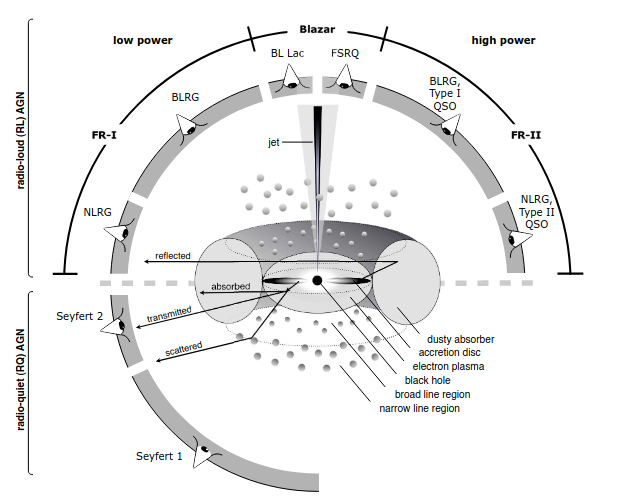
\includegraphics[width=\linewidth]{Plots/appendix/agn.png}
    \caption{This diagram shows the unified AGN scheme \cite{agn}. With blazars, the observer looks more or less directly into the jet of the AGN.}
    \label{fig:agn}
\end{figure}

\section{Theory}

This scheme is designed to facilitate understanding of sensitivity and discovery potential.

\begin{figure}
  \begin{tikzpicture}[
declare function={gamma(\z)=
2.506628274631*sqrt(1/\z)+ 0.20888568*(1/\z)^(1.5)+ 0.00870357*(1/\z)^(2.5)- (174.2106599*(1/\z)^(3.5))/25920- (715.6423511*(1/\z)^(4.5))/1244160)*exp((-ln(1/\z)-1)*\z;},
declare function={gammapdf(\x,\k,\theta) = 1/(\theta^\k)*1/(gamma(\k))*\x^(\k-1)*exp(-\x/\theta);}]
\begin{axis}[ymode=log, ymin=0,
no markers, domain=0:9, samples=100,
axis lines=left, xlabel=$\text{TS}$, ylabel=$\#\text{trials}$,
y label style={at={(axis description cs:-0.1,.5)},anchor=north},
x label style={dashed,at={(axis description cs:0.95,-0.1)},anchor=west},
height=5cm, width=9cm,
xtick={6,14.87}, ytick=\empty,
xticklabels={$\text{bg median}$,$5\sigma$},
%xticklabels={$\bar n (\theta_t)$},
enlargelimits=false, clip=false,% axis on top,
grid = major]
\addplot [very thick,cyan!20!black,domain=0:20, draw=none] {gammapdf(x,0.2,5)};
\addplot [very thick,cyan!20!black,domain=0.5:19.5] {gammapdf(x,0.2,5)};
%\addplot [domain= 0.5:4.5]{gauss(2.5,0.6,2)};
%\addplot [fill=cyan!20, draw=none, domain=0:6.0] {gammapdf(x,2,2)} \closedcycle;
%\addplot [very thick, fill=white!20!white, draw=none, domain=6.01:20] {gammapdf(x,2,2)} \closedcycle;
\end{axis}
\node at (2.5,1.7) {\begin{tikzpicture} \begin{axis}[hide axis,enlargelimits=false, ymax = 1,height=5cm, width=4cm,domain=2.65:3.35]\addplot [domain= 2.65:3.35,smooth,thick,green]{gauss(3,0.1,0.2)}; \end{axis} \end{tikzpicture}};
\node at (5.5,1.7) {\begin{tikzpicture} \begin{axis}[hide axis,enlargelimits=false, ymax = 1,height=5cm, width=3.5cm,domain=2.7:3.3]\addplot [domain= 2.7:3.3,smooth,thick,red]{gauss(3,0.07,0.14)}; \end{axis} \end{tikzpicture}};
\node[green] at (2.7,3) {$\xrightarrow{\text{90\%}}$};
\node[red] at (6,3) {$\xrightarrow{\text{50\%}}$};
\node at (0.5,3) {$\text{bg}$};
\node[green] at (2.7,4) {$\text{sensitivity}$};
\node[red] at (6,4) {$\text{discovery}$};
\end{tikzpicture}
\caption{Schematic showing the conditions to calculate the sensitivity and discovery potential. The background test statistic is shown in black, the signal test statistic satisfying the sensitivity conditions in green and the one for the discovery potential in red. Note that the curves dont actually look like these shown here. They have been simplified for explanatory purpose.}
\label{fig:sens_disc_schem}
\end{figure}

\section{Sources}

\begin{figure}
    \centering
    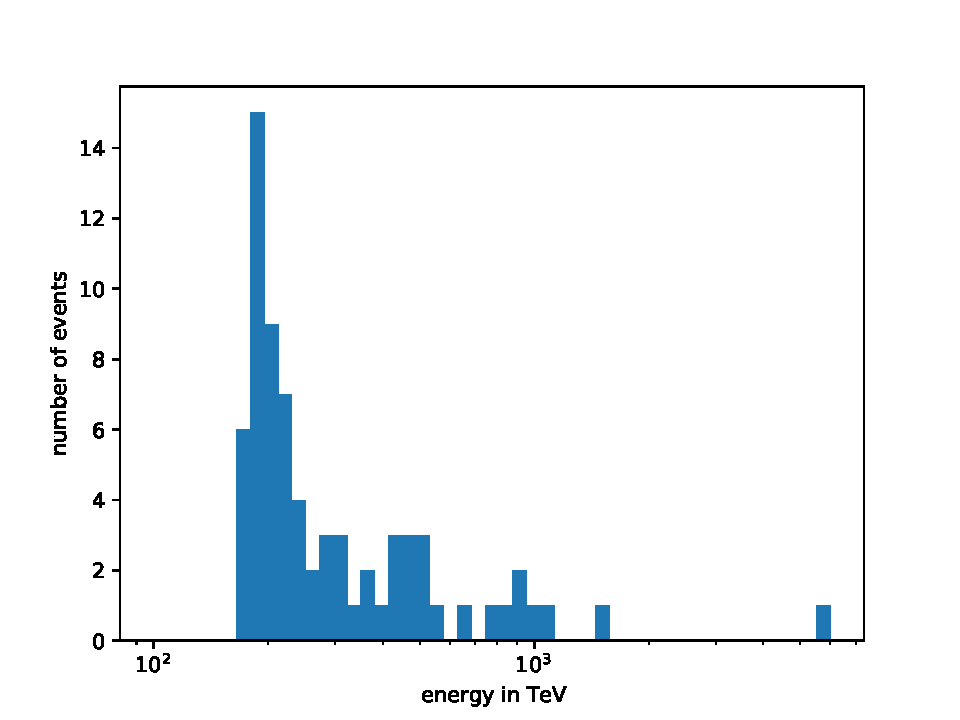
\includegraphics[width=\linewidth]{Plots/appendix/sources_energy.pdf}
    \caption{Histogram of the energy of the used sources seen in table \ref{tab:sources} in $\si{\tera\electronvolt}$.}
    \label{fig:sources_energy}
\end{figure}

\begin{table}
  \centering
  \caption{Table of the sources used in the time-dependent analysis. Additionally the signalness parameter is shown after which the sources were selected.}
  \label{tab:sources_time_dep}
  \begin{tabular}{ccrrc}
    \toprule
    Nr. & MJD &  $\delta$ in $\si{\degree}$ & $\alpha$ in $\si{\degree}$ & signalness in $\si{\percent}$ \\
    \toprule
      11 & 56819.20 & 11.45 & 110.65 & 99.70 \\ 12 & 56470.11 & 14.17 & 93.74 & 93.80 \\ 13 & 57951.82 & 25.16 & 208.39 & 86.60 \\ 16 & 58063.78 & 7.44 & 340.14 & 97.50 \\ 29 & 57340.87 & 12.71 & 76.16 & 95.70 \\ 37 & 55911.28 & 18.88 & 36.74 & 94.60 \\ 42 & 56226.60 & 27.91 & 169.80 & 92.60 \\ 43 & 56666.50 & 33.02 & 293.12 & 92.70 \\ 58 & 57478.57 & 15.48 & 151.22 & 85.10 \\ 63 & 56211.77 & -2.28 & 205.14 & 84.20 \\ 
    \toprule
  \end{tabular}
\end{table}

\section{Time-Integrated Search}

\begin{table}
  \centering
  \caption{Table of the number of injected signal events used for the time integrated analysis.}
  \label{tab:sig_time_int_table}
  \begin{tabular}{r}
    \toprule
    $n_\text{S}$ injected \\
    \toprule
      0.0 \\ 7.5 \\ 15.0 \\ 22.5 \\ 30.0 \\ 36.0 \\ 57.0 \\ 78.0 \\ 99.0 \\ 120.0 \\ 141.0 \\ 194.2 \\ 247.4 \\ 300.7 \\ 353.9 \\ 407.1 \\ 460.3 \\ 513.6 \\ 566.8 \\ 620.0 \\ 
    \toprule
  \end{tabular}
\end{table}

\begin{table}
  \caption{Table of the number of trials for each spectral index $\gamma$ and number of injected signal events $n_\text{sig}$, running $\num{10}$ jobs with $\num{5e3}$ trials per set of parameter pairs $\gamma$ and $n_\text{sig}$. Some jobs fail due to technical reasons.}
  \label{tab:trials_sig_time_int_table}
  \begin{subtable}{\linewidth}
  \centering
  \begin{tabular}{p{.9cm}|rrrrrrrrrr}
    \toprule
    \: $n_\text{sig}$ \newline $\gamma$ \: & 0.0 & 7.5 & 15.0 & 22.5 & 30.0 & 36.0 & 57.0 & 78.0 & 99.0 & 141.0 \\ 
    \toprule
    1.50 & 50000 & 50000 & 50000 & 50000 & 50000 & 50000 & 50000 & 50000 & 50000 & 50000 \\ 1.75 & 50000 & 50000 & 50000 & 50000 & 50000 & 50000 & 50000 & 50000 & 50000 & 50000 \\ 2.00 & 50000 & 50000 & 50000 & 50000 & 50000 & 50000 & 50000 & 50000 & 50000 & 50000 \\ 2.25 & 50000 & 45000 & 45000 & 45000 & 50000 & 45000 & 50000 & 50000 & 50000 & 50000 \\ 2.50 & 50000 & 50000 & 50000 & 50000 & 50000 & 50000 & 50000 & 50000 & 50000 & 50000 \\ 2.75 & 50000 & 50000 & 45000 & 45000 & 50000 & 50000 & 50000 & 40000 & 50000 & 40000 \\ 3.00 & 50000 & 50000 & 50000 & 50000 & 50000 & 45000 & 50000 & 50000 & 50000 & 50000 \\ 
    \toprule
  \end{tabular}
\end{subtable}
\begin{subtable}{\linewidth}
\centering
  \begin{tabular}{p{.9cm}|rrrrrrrrrr}
    \toprule
    \: $n_\text{sig}$ \newline $\gamma$ \: & 141.0 & 194.2 & 247.4 & 300.7 & 353.9 & 407.1 & 460.3 & 513.6 & 566.8 & 620.0 \\ 
    \toprule
    1.50 & 50000 & 50000 & 50000 & 50000 & 50000 & 50000 & 50000 & 50000 & 50000 & 50000 \\ 1.75 & 50000 & 50000 & 50000 & 50000 & 50000 & 50000 & 50000 & 50000 & 50000 & 45000 \\ 2.00 & 50000 & 50000 & 50000 & 50000 & 50000 & 50000 & 50000 & 50000 & 50000 & 50000 \\ 2.25 & 50000 & 50000 & 50000 & 50000 & 50000 & 50000 & 50000 & 50000 & 50000 & 50000 \\ 2.50 & 50000 & 50000 & 50000 & 50000 & 50000 & 50000 & 50000 & 50000 & 50000 & 40000 \\ 2.75 & 50000 & 50000 & 50000 & 50000 & 50000 & 50000 & 50000 & 50000 & 50000 & 50000 \\ 3.00 & 50000 & 50000 & 45000 & 50000 & 50000 & 50000 & 50000 & 50000 & 50000 & 50000 \\ 
    \toprule
  \end{tabular}
  \end{subtable}
\end{table}

\section{Time-Dependent Search} \label{sec:time_dep_search_appendix}

In this chapter the complete results for all $\num{10}$ sources can be found.

\subsection{Background Trials}

\begin{figure}
    \centering
    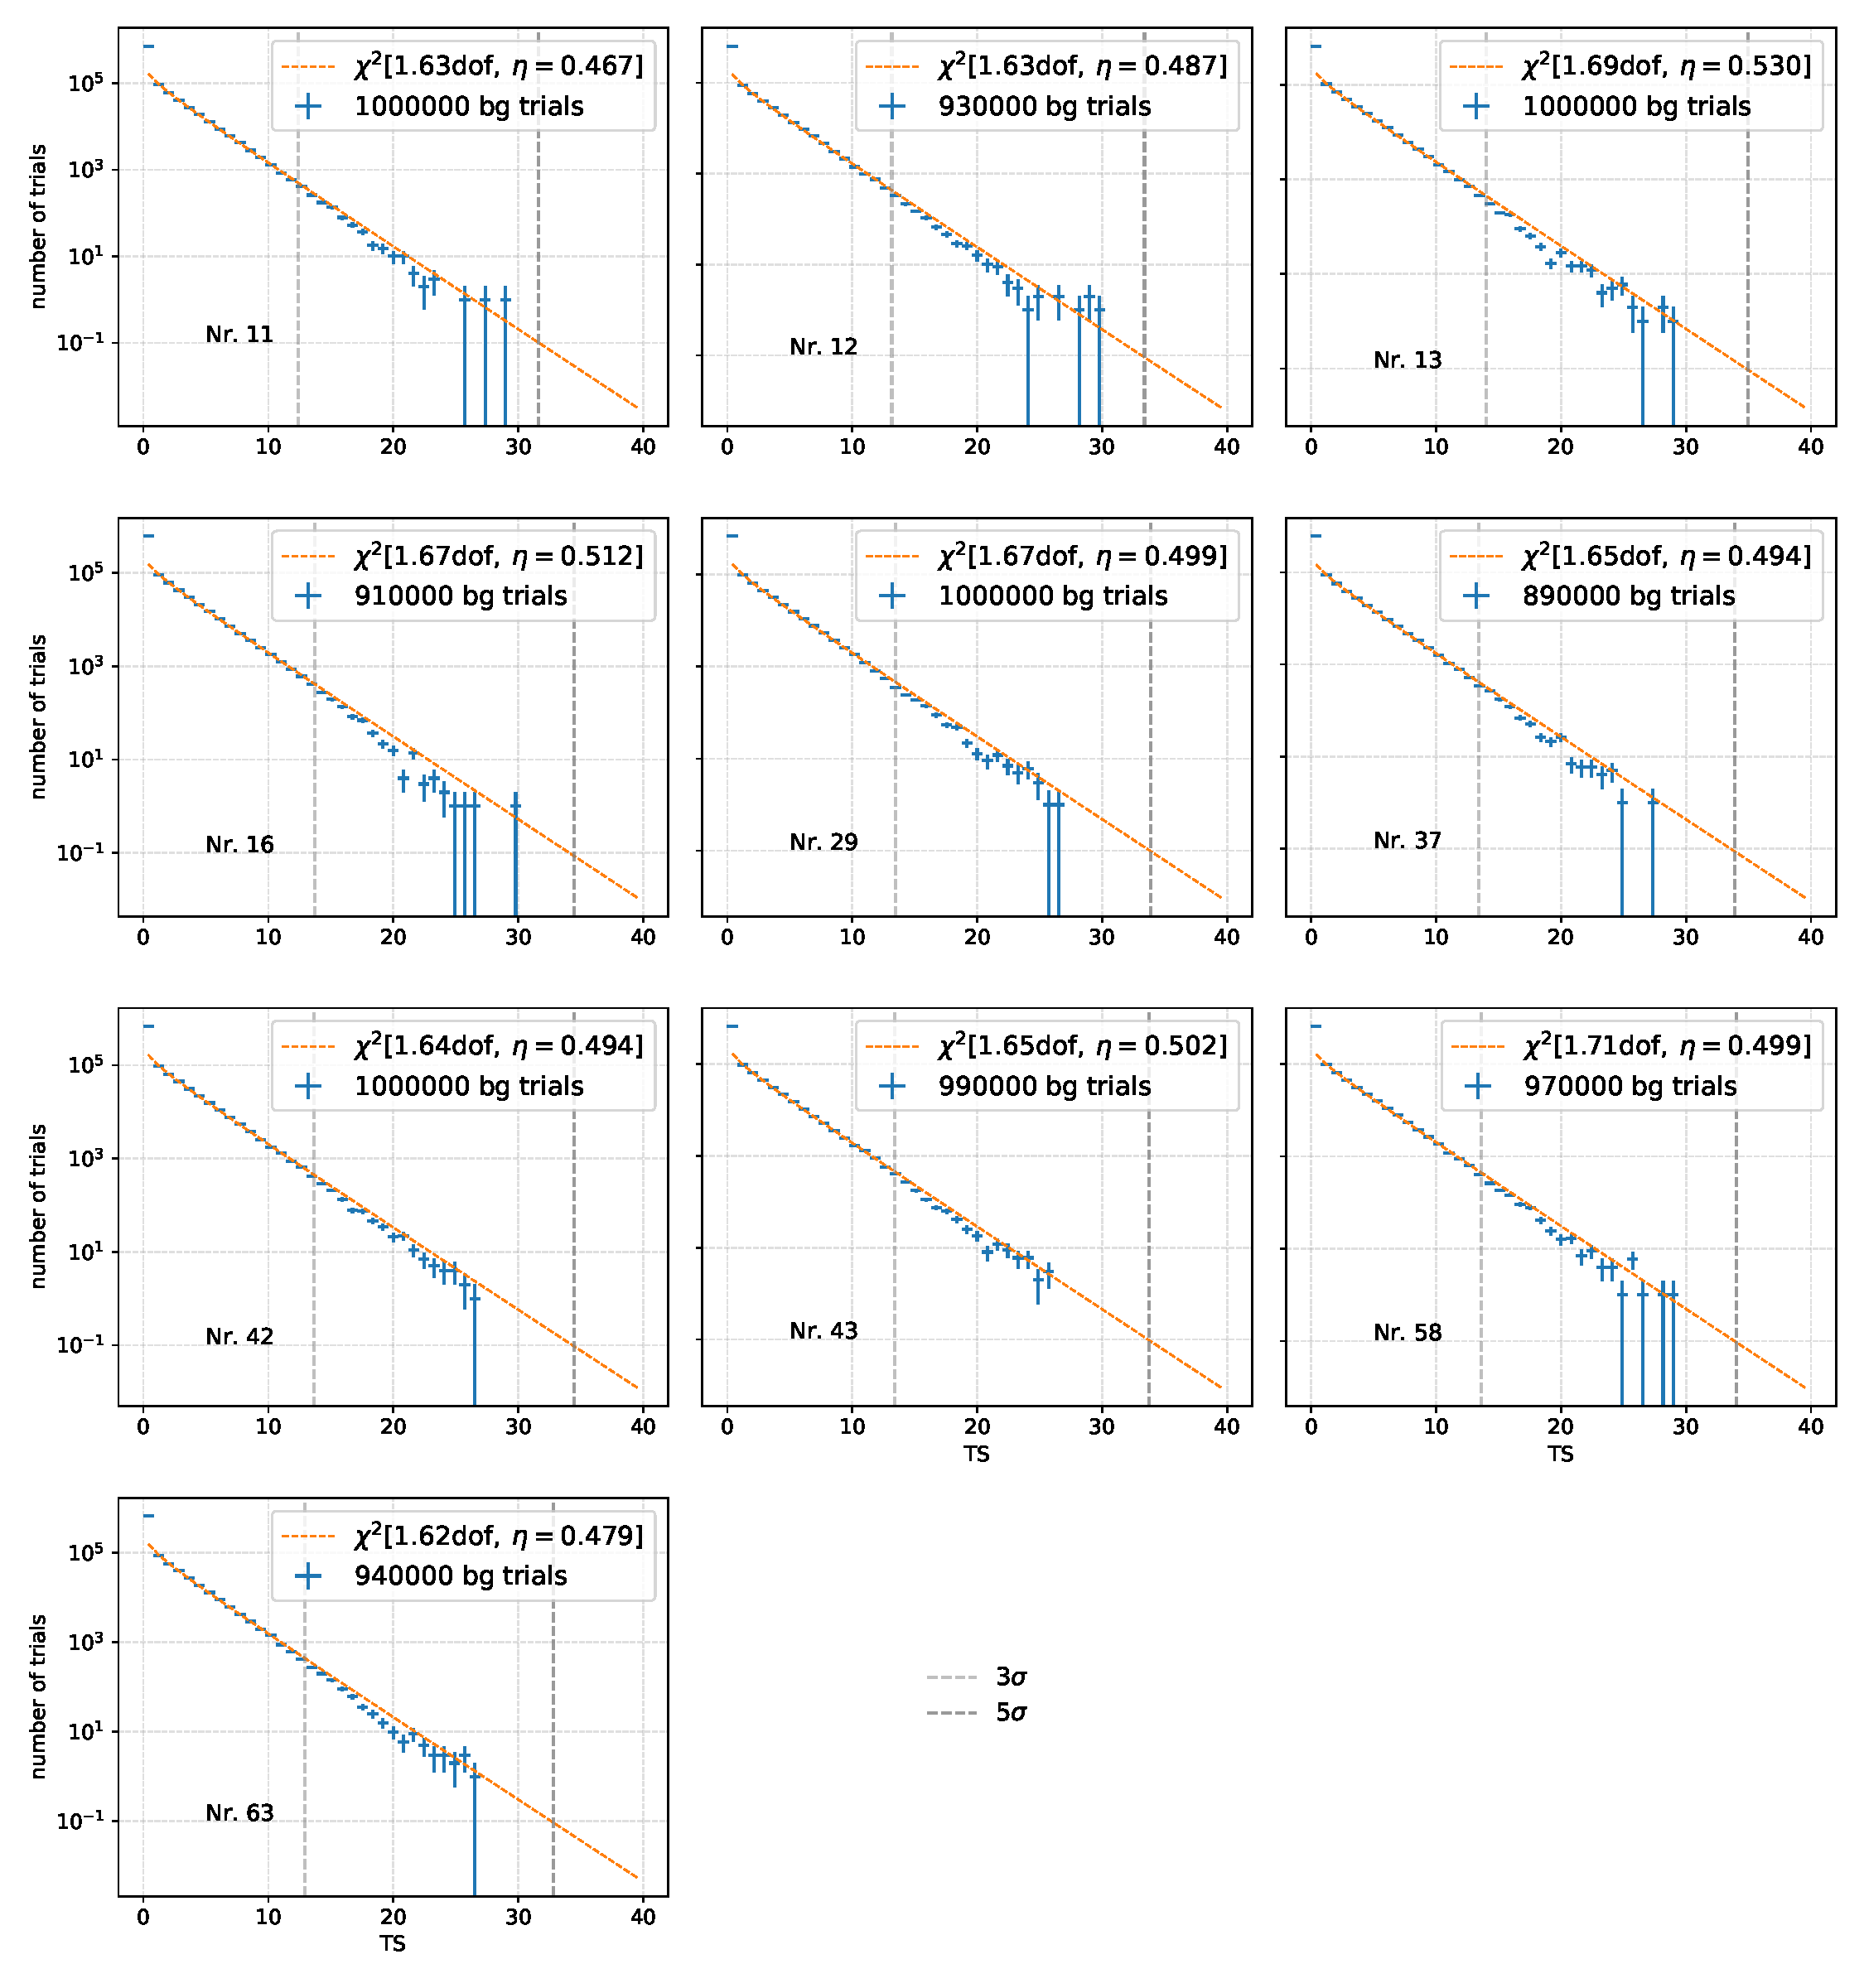
\includegraphics[width=\linewidth-2cm]{Plots/05_csky/9_years_gfu_gold_time_dep_bg_t0.pdf}
    \caption{Histograms of the background test statistic values for all $\num{10}$ sources used in the time-dependent analysis. Shown are also the number of degrees of freedom $dof$ and the ratio of positive and negative values $\eta$. The id of the sources corresponds to table \ref{tab:sources} or \ref{tab:sources_time_dep} respectively.}
    \label{fig:bg_trials_time_dep}
\end{figure}

\begin{figure}
    \centering
    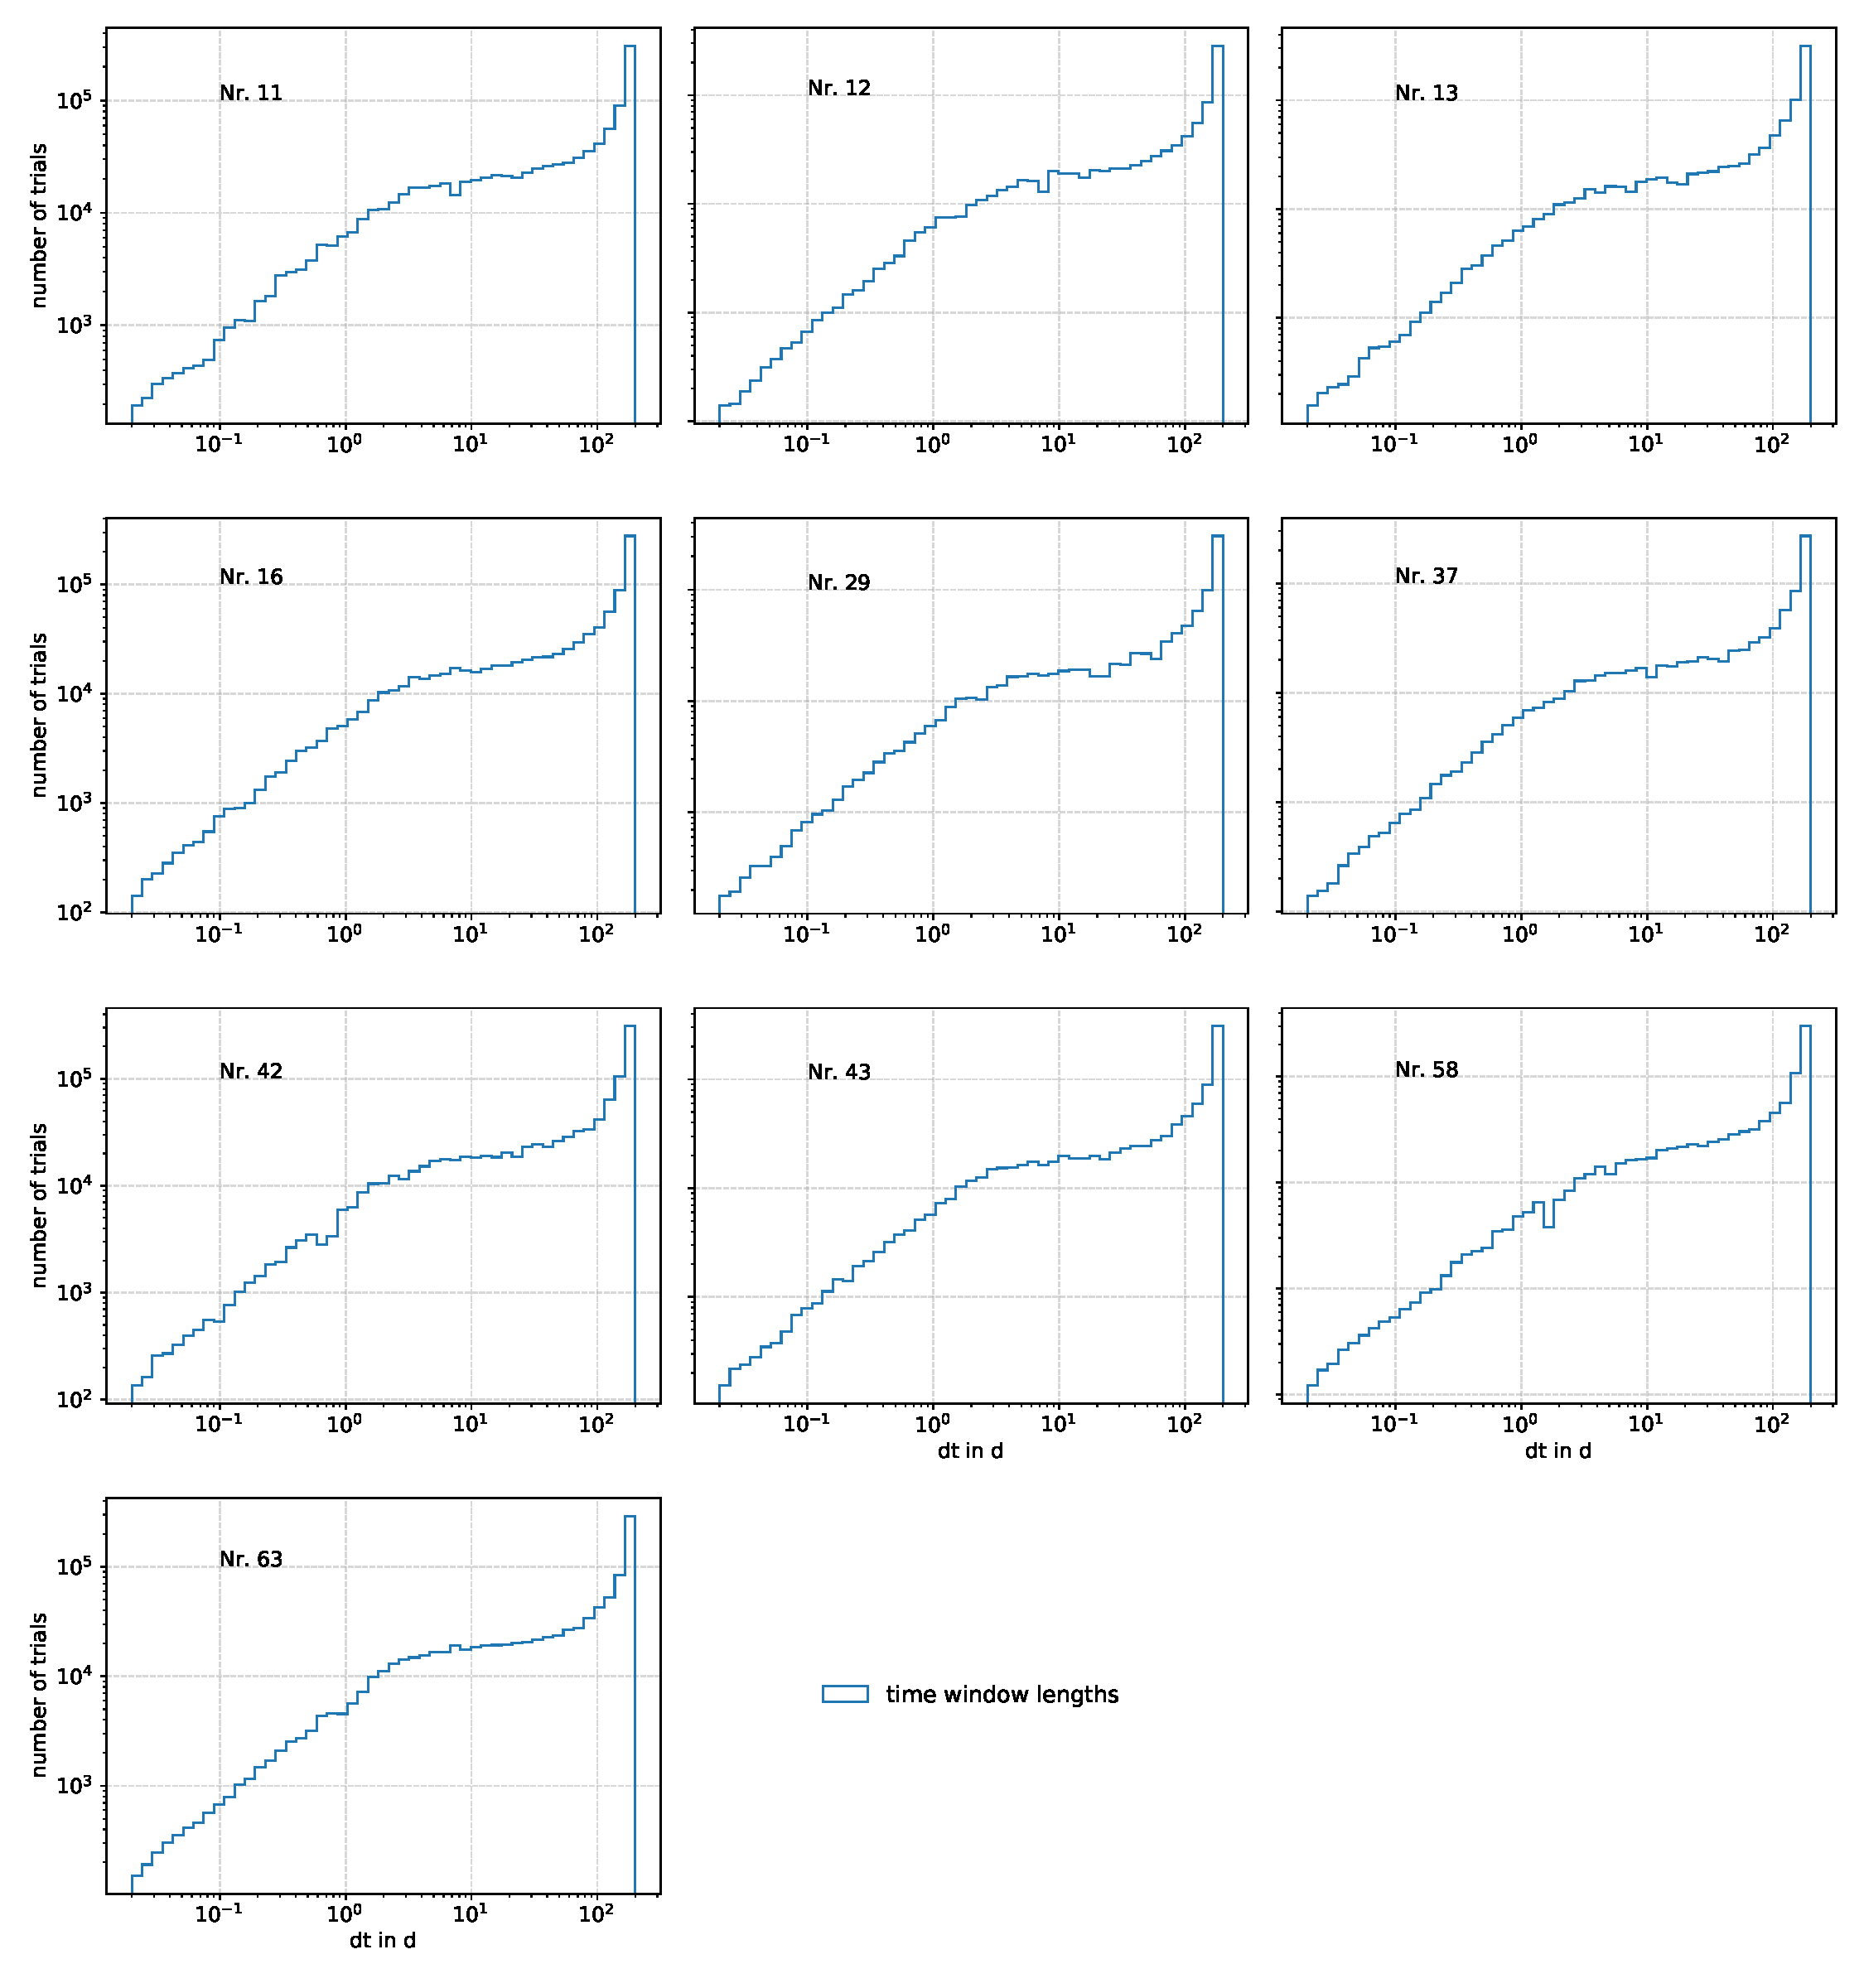
\includegraphics[width=\linewidth]{Plots/05_csky/9_years_gfu_gold_time_dep_bg_dt.pdf}
    \caption{Histograms of the background time window lengths $dt$ in days of all $\num{10}$ sources for the time-dependent analysis.}
    \label{fig:bg_trials_time_dep_time_windows}
\end{figure}

\begin{figure}
    \centering
    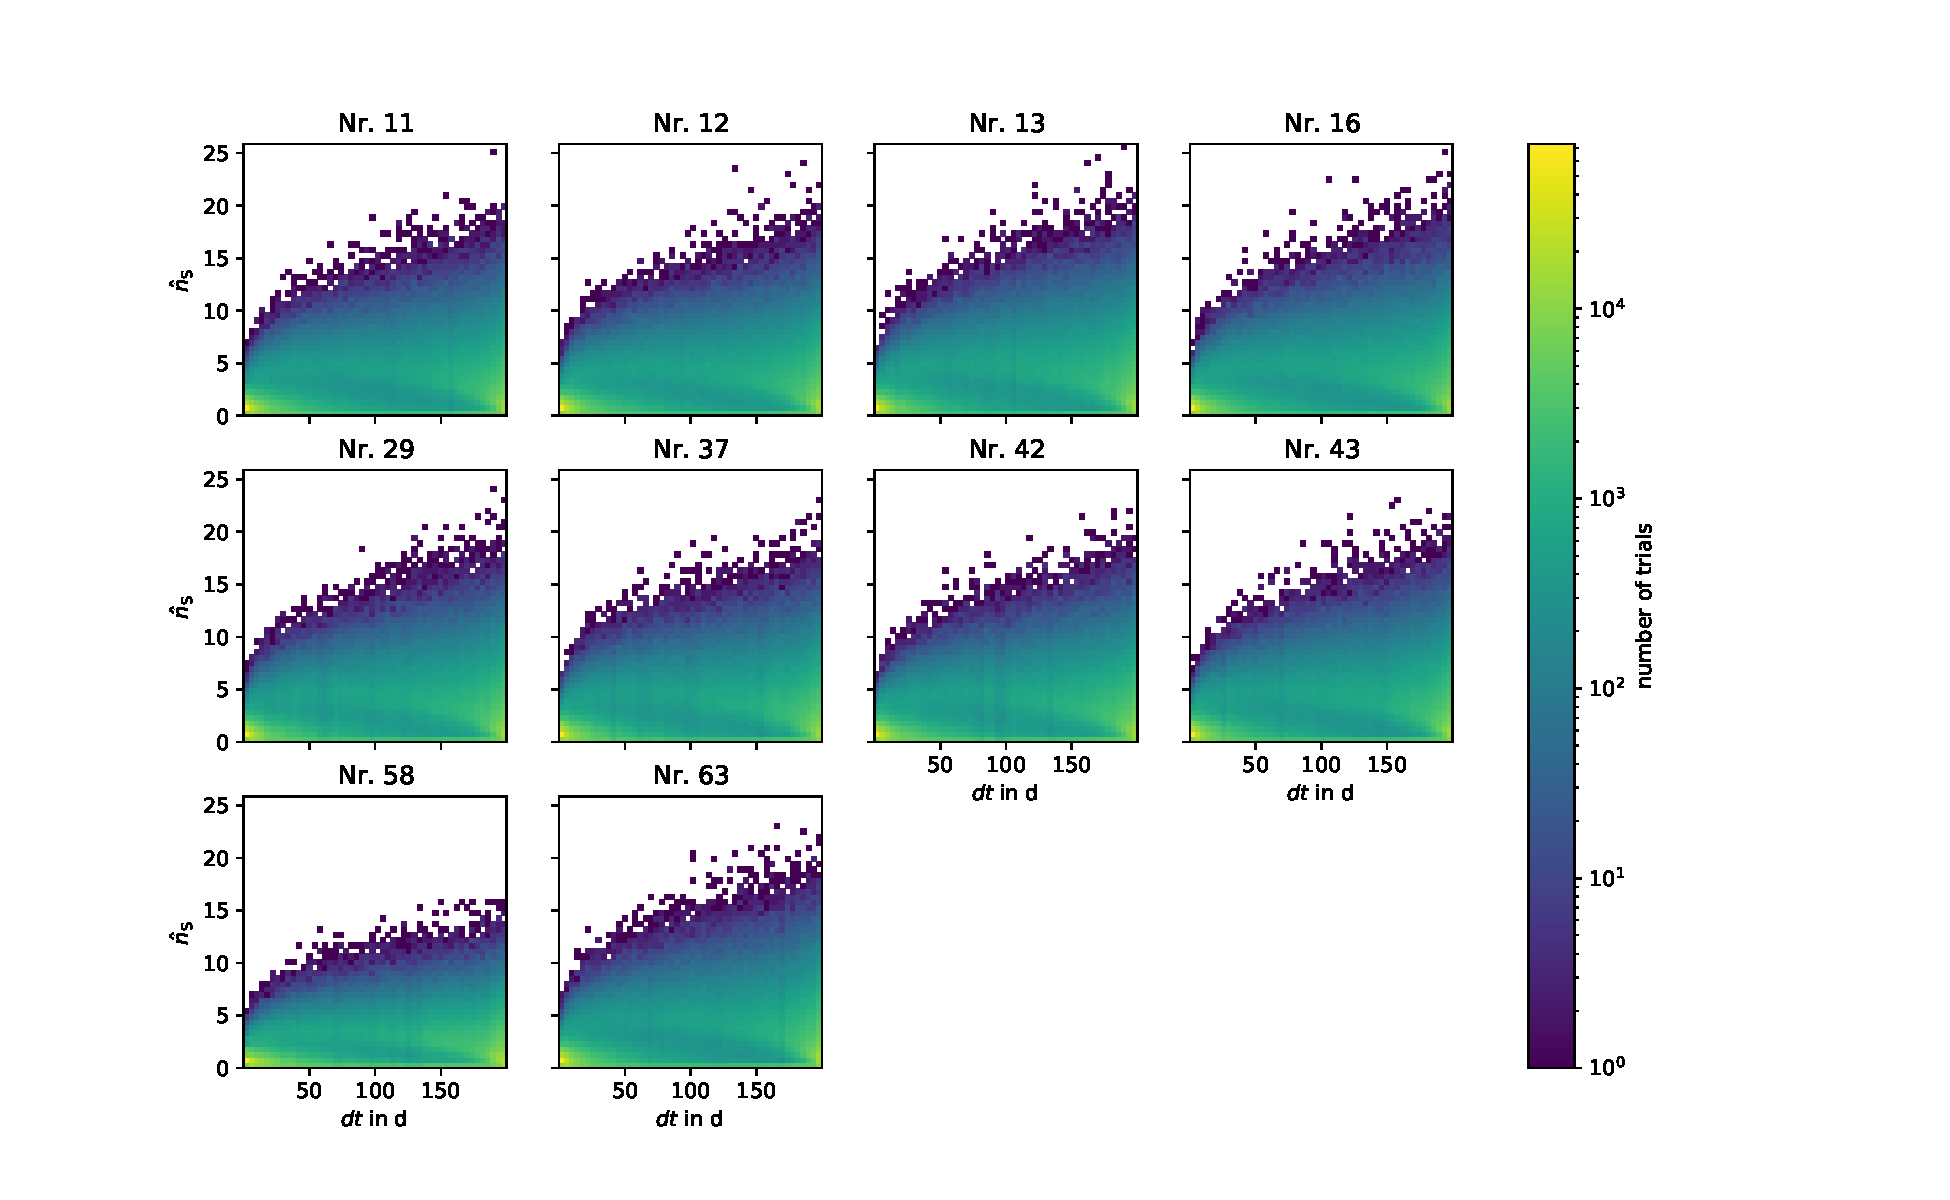
\includegraphics[width=\linewidth]{Plots/05_csky/time_window_ns_bg_time_dep.pdf}
    \caption{Histograms of the fitted number of signal events $\hat{n}_\text{S}$ in dependence of the time window lengths $dt$ in days of the background trials for the time-dependent analysis for all $\num{10}$ sources.}
    \label{fig:bg_trials_time_dep_time_windows_ns}
\end{figure}

\newpage
\subsection{Signal Trials}

\begin{table}
  \centering
  \caption{Table of the number of trials for each spectral index source index number and number of injected signal events $n_\text{sig}$, running $\num{5}$ jobs with $\num{e4}$ trials per set of parameter pairs of source and $n_\text{sig}$. Some jobs fail due to technical reasons.}
  \label{tab:trials_sig_time_dep_table}
  \begin{tabular}{>{\centering\arraybackslash}p{.9cm}|%
                    cccccccccc}
    \toprule
    \: Nr. \newline $n_\text{sig}$ \: & 11 & 12 & 13 & 16 & 29 & 37 & 42 & 43 & 58 & 63 \\ 
    \toprule
    0.0 & 50000 & 50000 & 50000 & 50000 & 50000 & 10000 & 40000 & 50000 & 50000 & 30000 \\ 1.1 & 50000 & 50000 & 50000 & 50000 & 50000 & 20000 & 40000 & 50000 & 50000 & 20000 \\ 2.2 & 50000 & 50000 & 50000 & 50000 & 50000 & 0 & 40000 & 50000 & 50000 & 30000 \\ 3.3 & 50000 & 50000 & 40000 & 50000 & 50000 & 50000 & 40000 & 50000 & 50000 & 30000 \\ 4.4 & 50000 & 50000 & 30000 & 50000 & 50000 & 40000 & 50000 & 50000 & 50000 & 10000 \\ 5.6 & 50000 & 40000 & 30000 & 50000 & 50000 & 40000 & 50000 & 50000 & 50000 & 20000 \\ 6.7 & 50000 & 40000 & 30000 & 50000 & 50000 & 50000 & 50000 & 50000 & 50000 & 50000 \\ 7.8 & 50000 & 50000 & 30000 & 50000 & 50000 & 50000 & 50000 & 50000 & 50000 & 50000 \\ 8.9 & 50000 & 50000 & 30000 & 20000 & 40000 & 50000 & 50000 & 50000 & 50000 & 40000 \\ 10.0 & 50000 & 50000 & 30000 & 40000 & 50000 & 50000 & 50000 & 50000 & 50000 & 50000 \\ 12.0 & 50000 & 50000 & 50000 & 30000 & 50000 & 50000 & 50000 & 50000 & 50000 & 50000 \\ 14.0 & 50000 & 50000 & 50000 & 20000 & 50000 & 50000 & 50000 & 50000 & 50000 & 50000 \\ 16.0 & 50000 & 40000 & 50000 & 30000 & 50000 & 50000 & 50000 & 50000 & 50000 & 50000 \\ 18.0 & 50000 & 50000 & 50000 & 40000 & 50000 & 50000 & 50000 & 50000 & 50000 & 50000 \\ 20.0 & 50000 & 50000 & 50000 & 40000 & 50000 & 40000 & 50000 & 50000 & 50000 & 40000 \\ 22.0 & 50000 & 50000 & 50000 & 50000 & 50000 & 30000 & 50000 & 50000 & 50000 & 50000 \\ 24.0 & 50000 & 50000 & 50000 & 50000 & 50000 & 30000 & 50000 & 50000 & 50000 & 50000 \\ 26.0 & 50000 & 50000 & 50000 & 50000 & 50000 & 30000 & 50000 & 50000 & 50000 & 50000 \\ 28.0 & 50000 & 50000 & 50000 & 50000 & 50000 & 40000 & 50000 & 50000 & 50000 & 50000 \\ 30.0 & 50000 & 50000 & 50000 & 50000 & 30000 & 20000 & 50000 & 50000 & 50000 & 50000 \\ 
    \toprule
  \end{tabular}
\end{table}

\begin{figure}
    \centering
    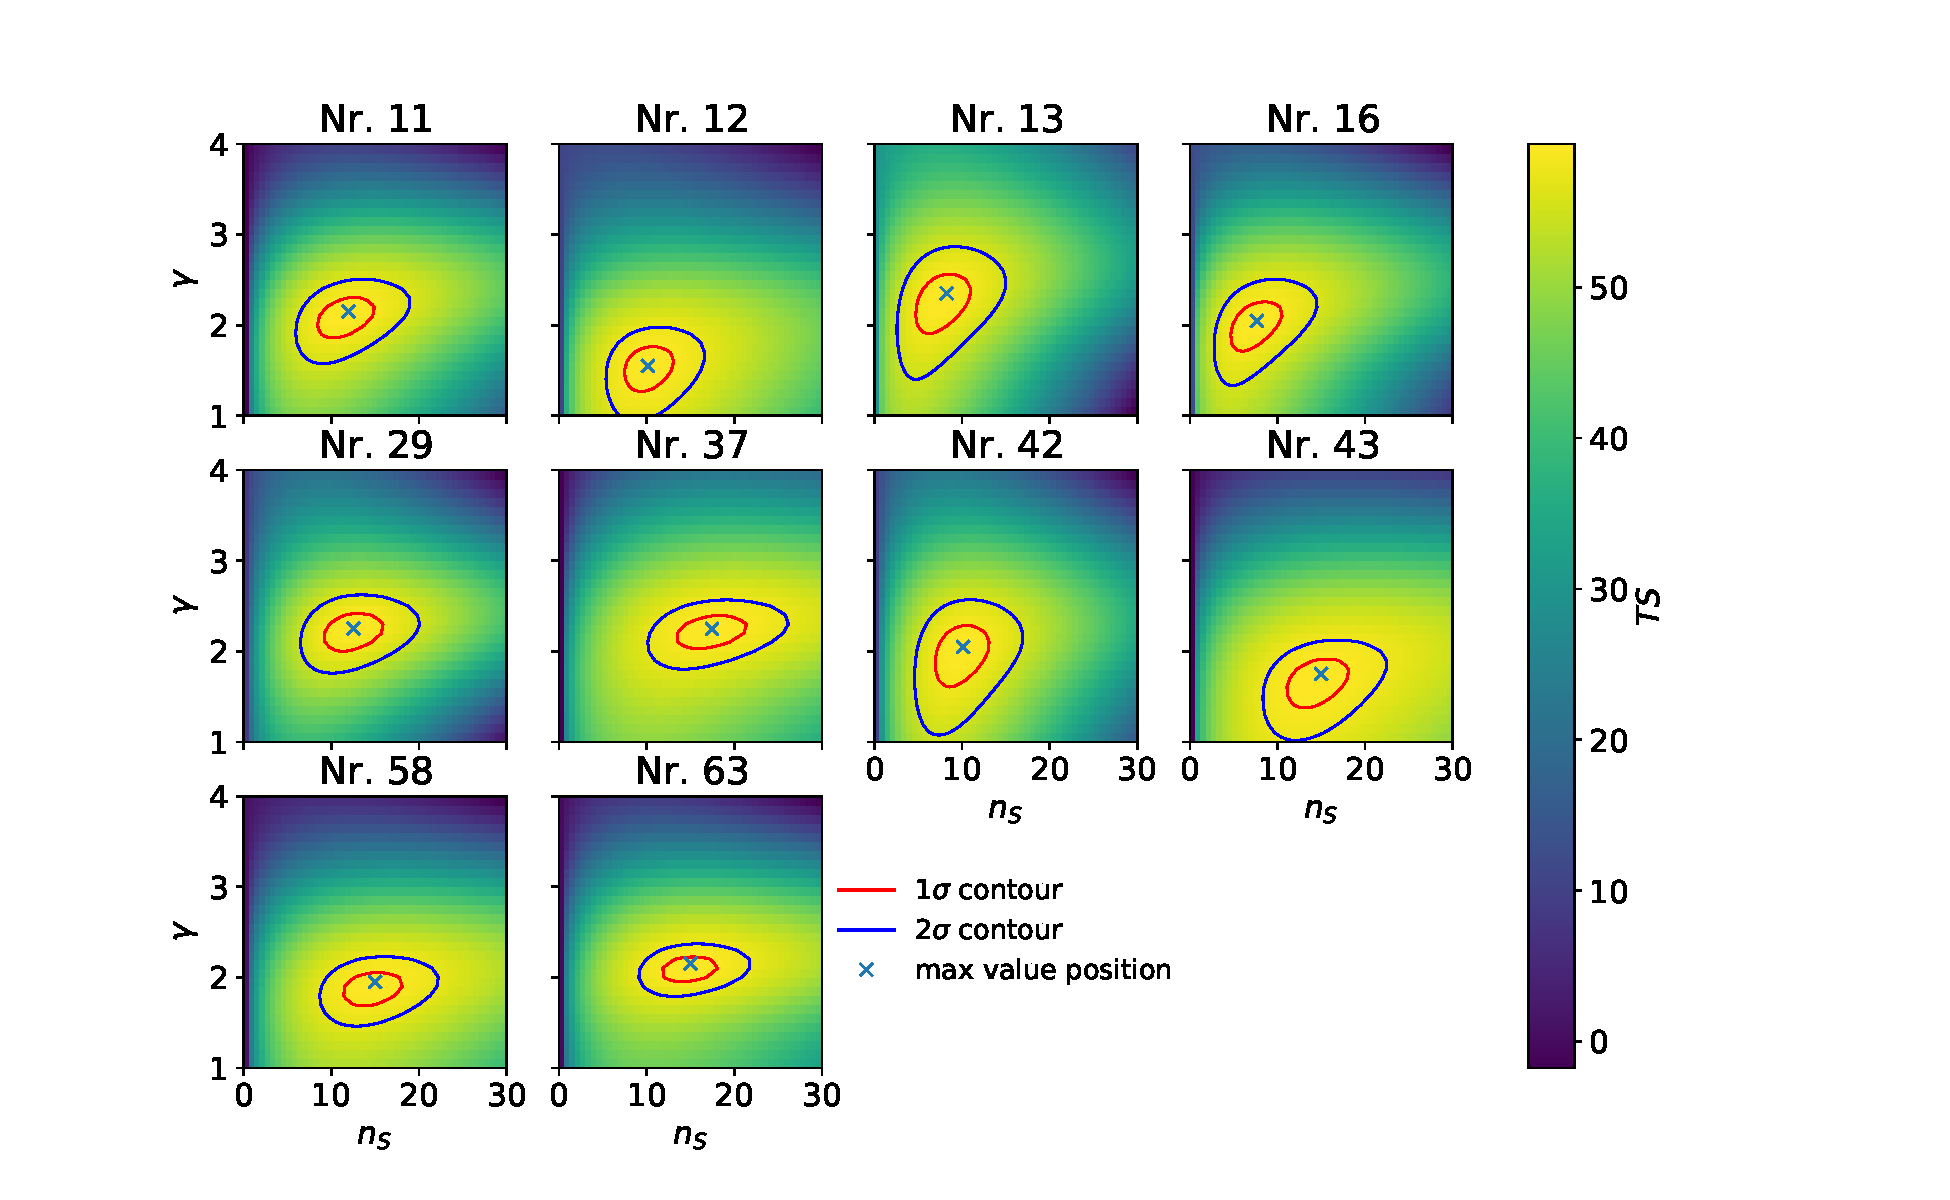
\includegraphics[width=\linewidth]{Plots/appendix/llh_scan.pdf}
    \caption{Scan of the likelihoodspace for all $\num{10}$ sources with a timewindow of $\SI{200}{\day}$ for the time-dependent analysis. The scan is in the spectral index $\gamma$ and the signal parameter $n_\text{S}$. The number of induced signal events is $n_S = \num{10}$ with a spectral index of $\gamma = 2$. The maximum test statistic value is marked in the plot including the contours of $\num{1}\sigma$ and $\num{2}\sigma$ and source number corresponds to table \ref{tab:sources}.}
    \label{fig:llh_scan_time_dep_all}
\end{figure}

\begin{figure}
    \centering
    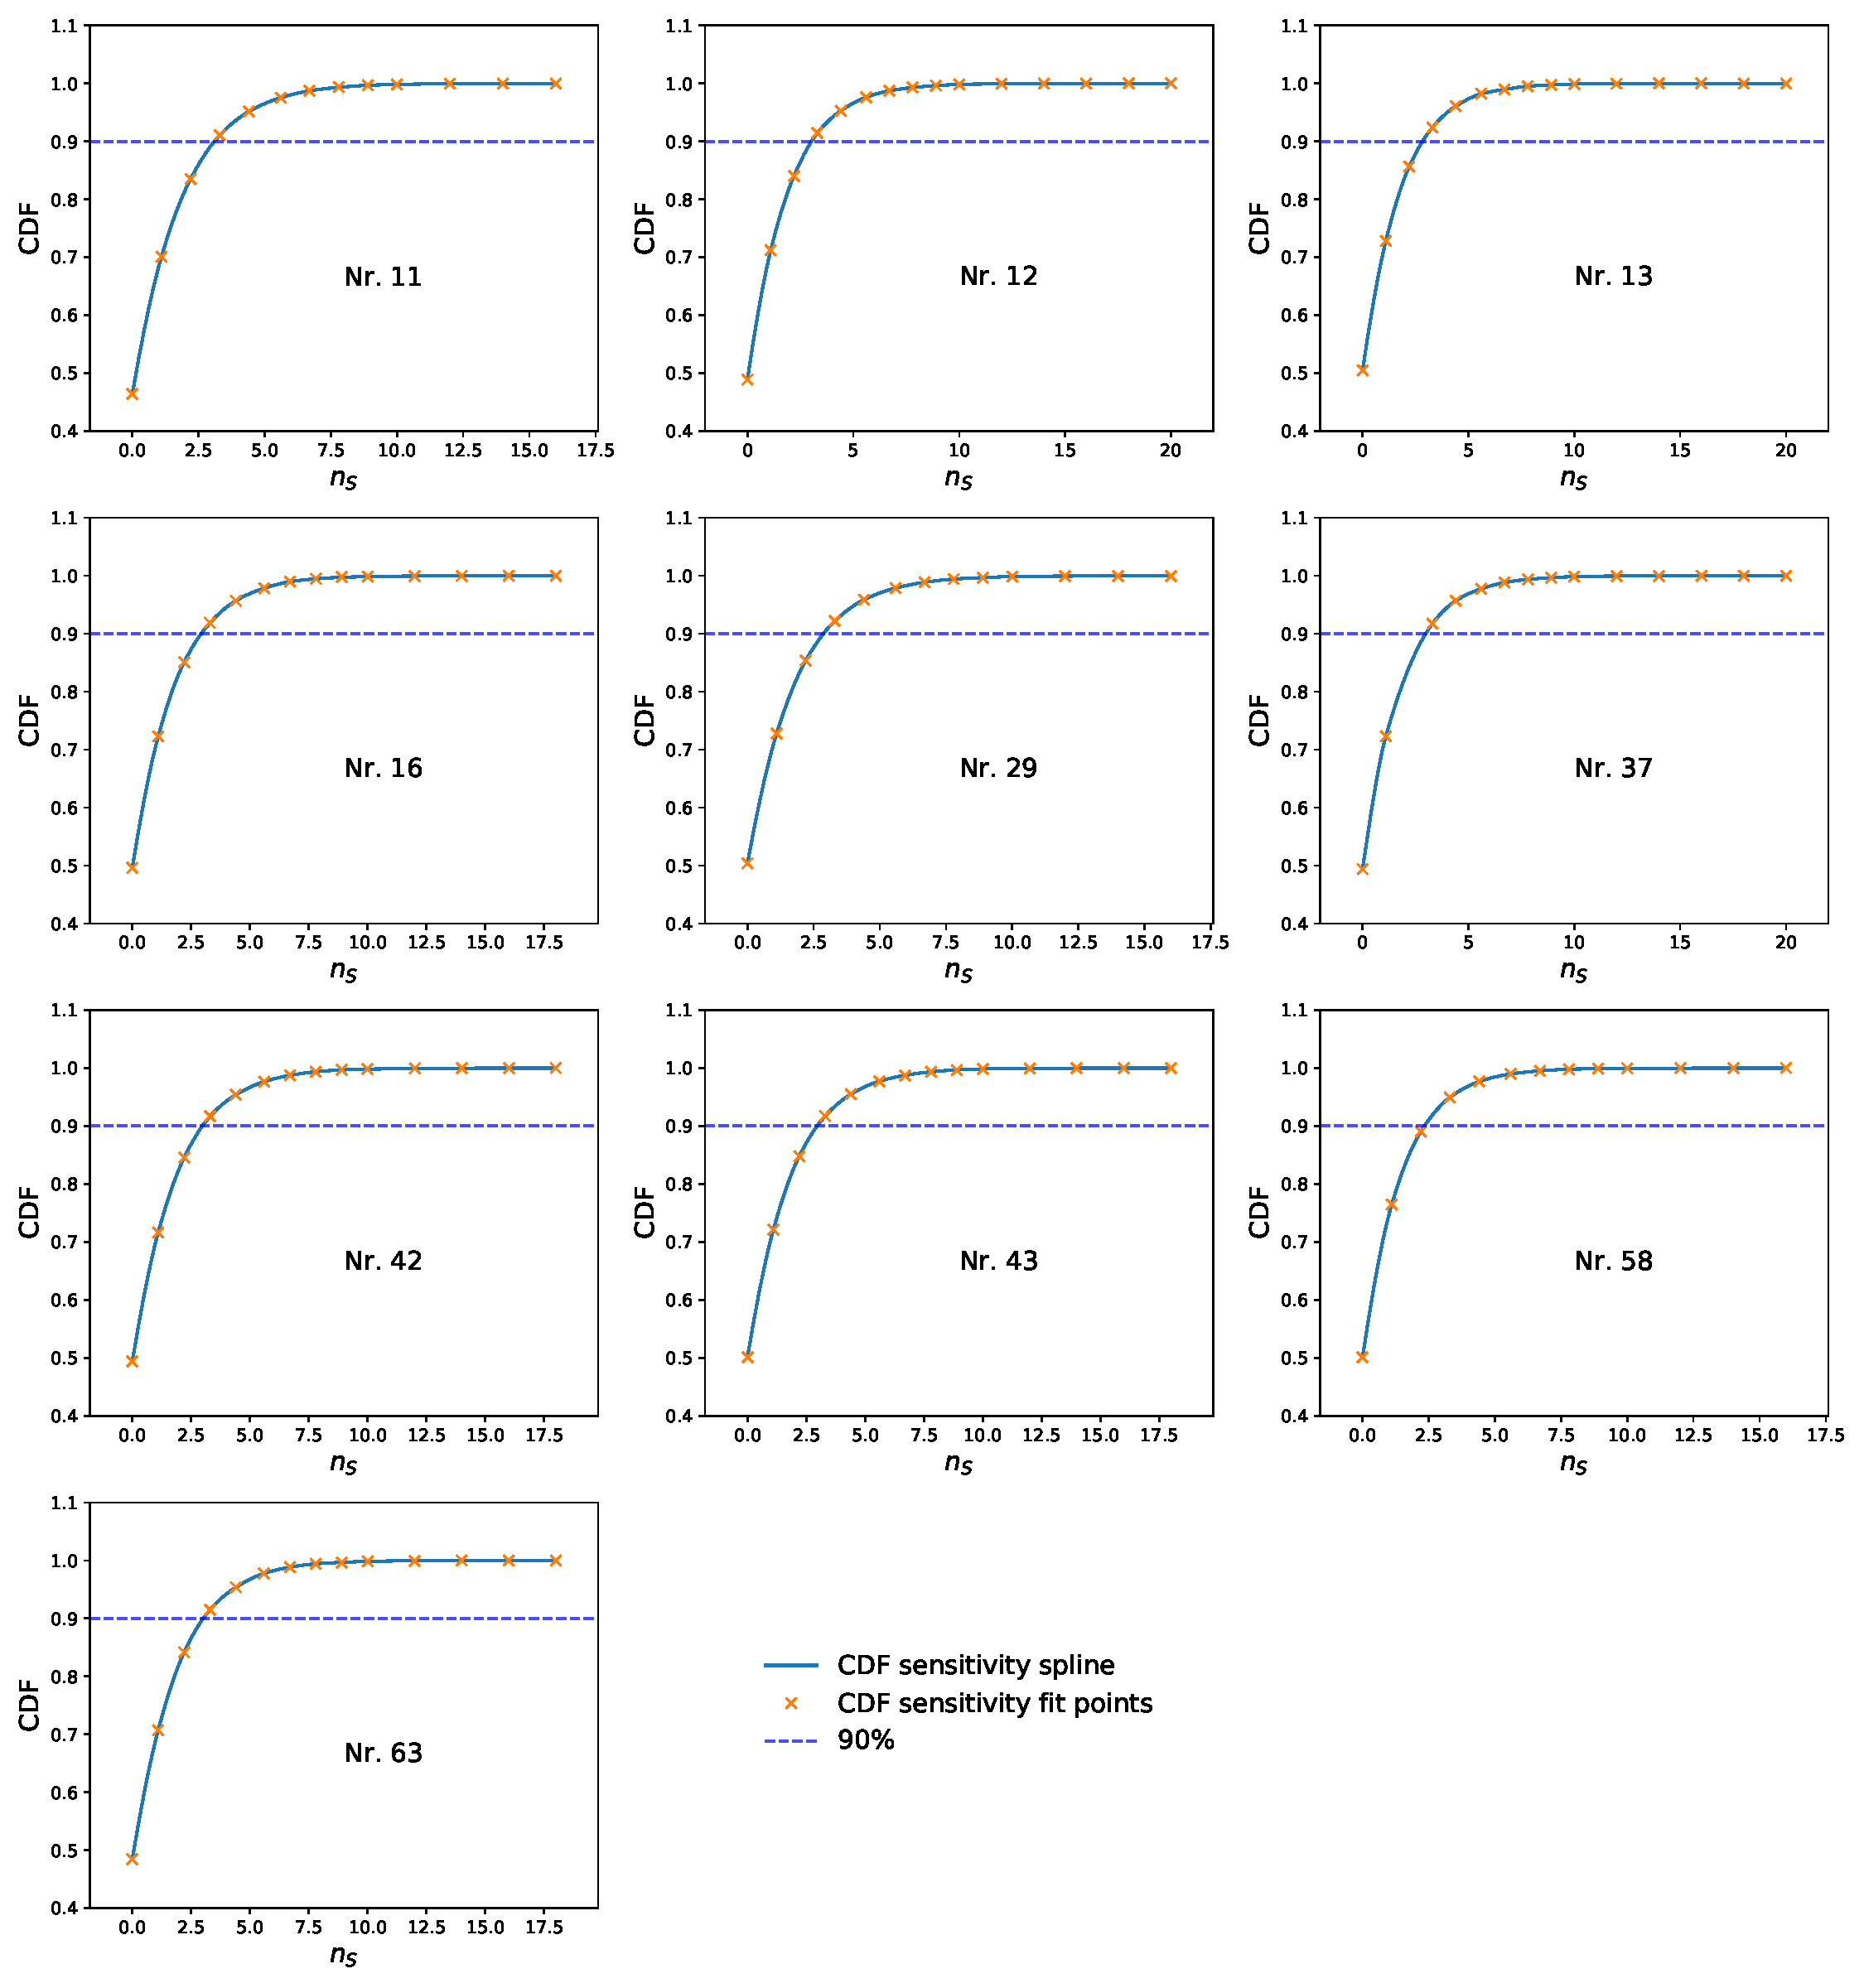
\includegraphics[width=\linewidth]{Plots/appendix/9_years_gfu_gold_time_dep_cdf_sens.pdf}
    \caption{Quantiles of the signal trials for the calculation of the discovery potential for the time-dependent analysis of all $\num{10}$ sources at a spectral index of $\gamma=\num{2}$. A $\chi^2$ CDF fit provides a more accurate estimate of the sought signal parameter $n_\text{S}$ which satisfies the condition of the sensitivity at $\SI{90}{\percent}$ represented via a dashed line.}
    \label{fig:time_dep_cdf_sens}
\end{figure}

\begin{figure}
    \centering
    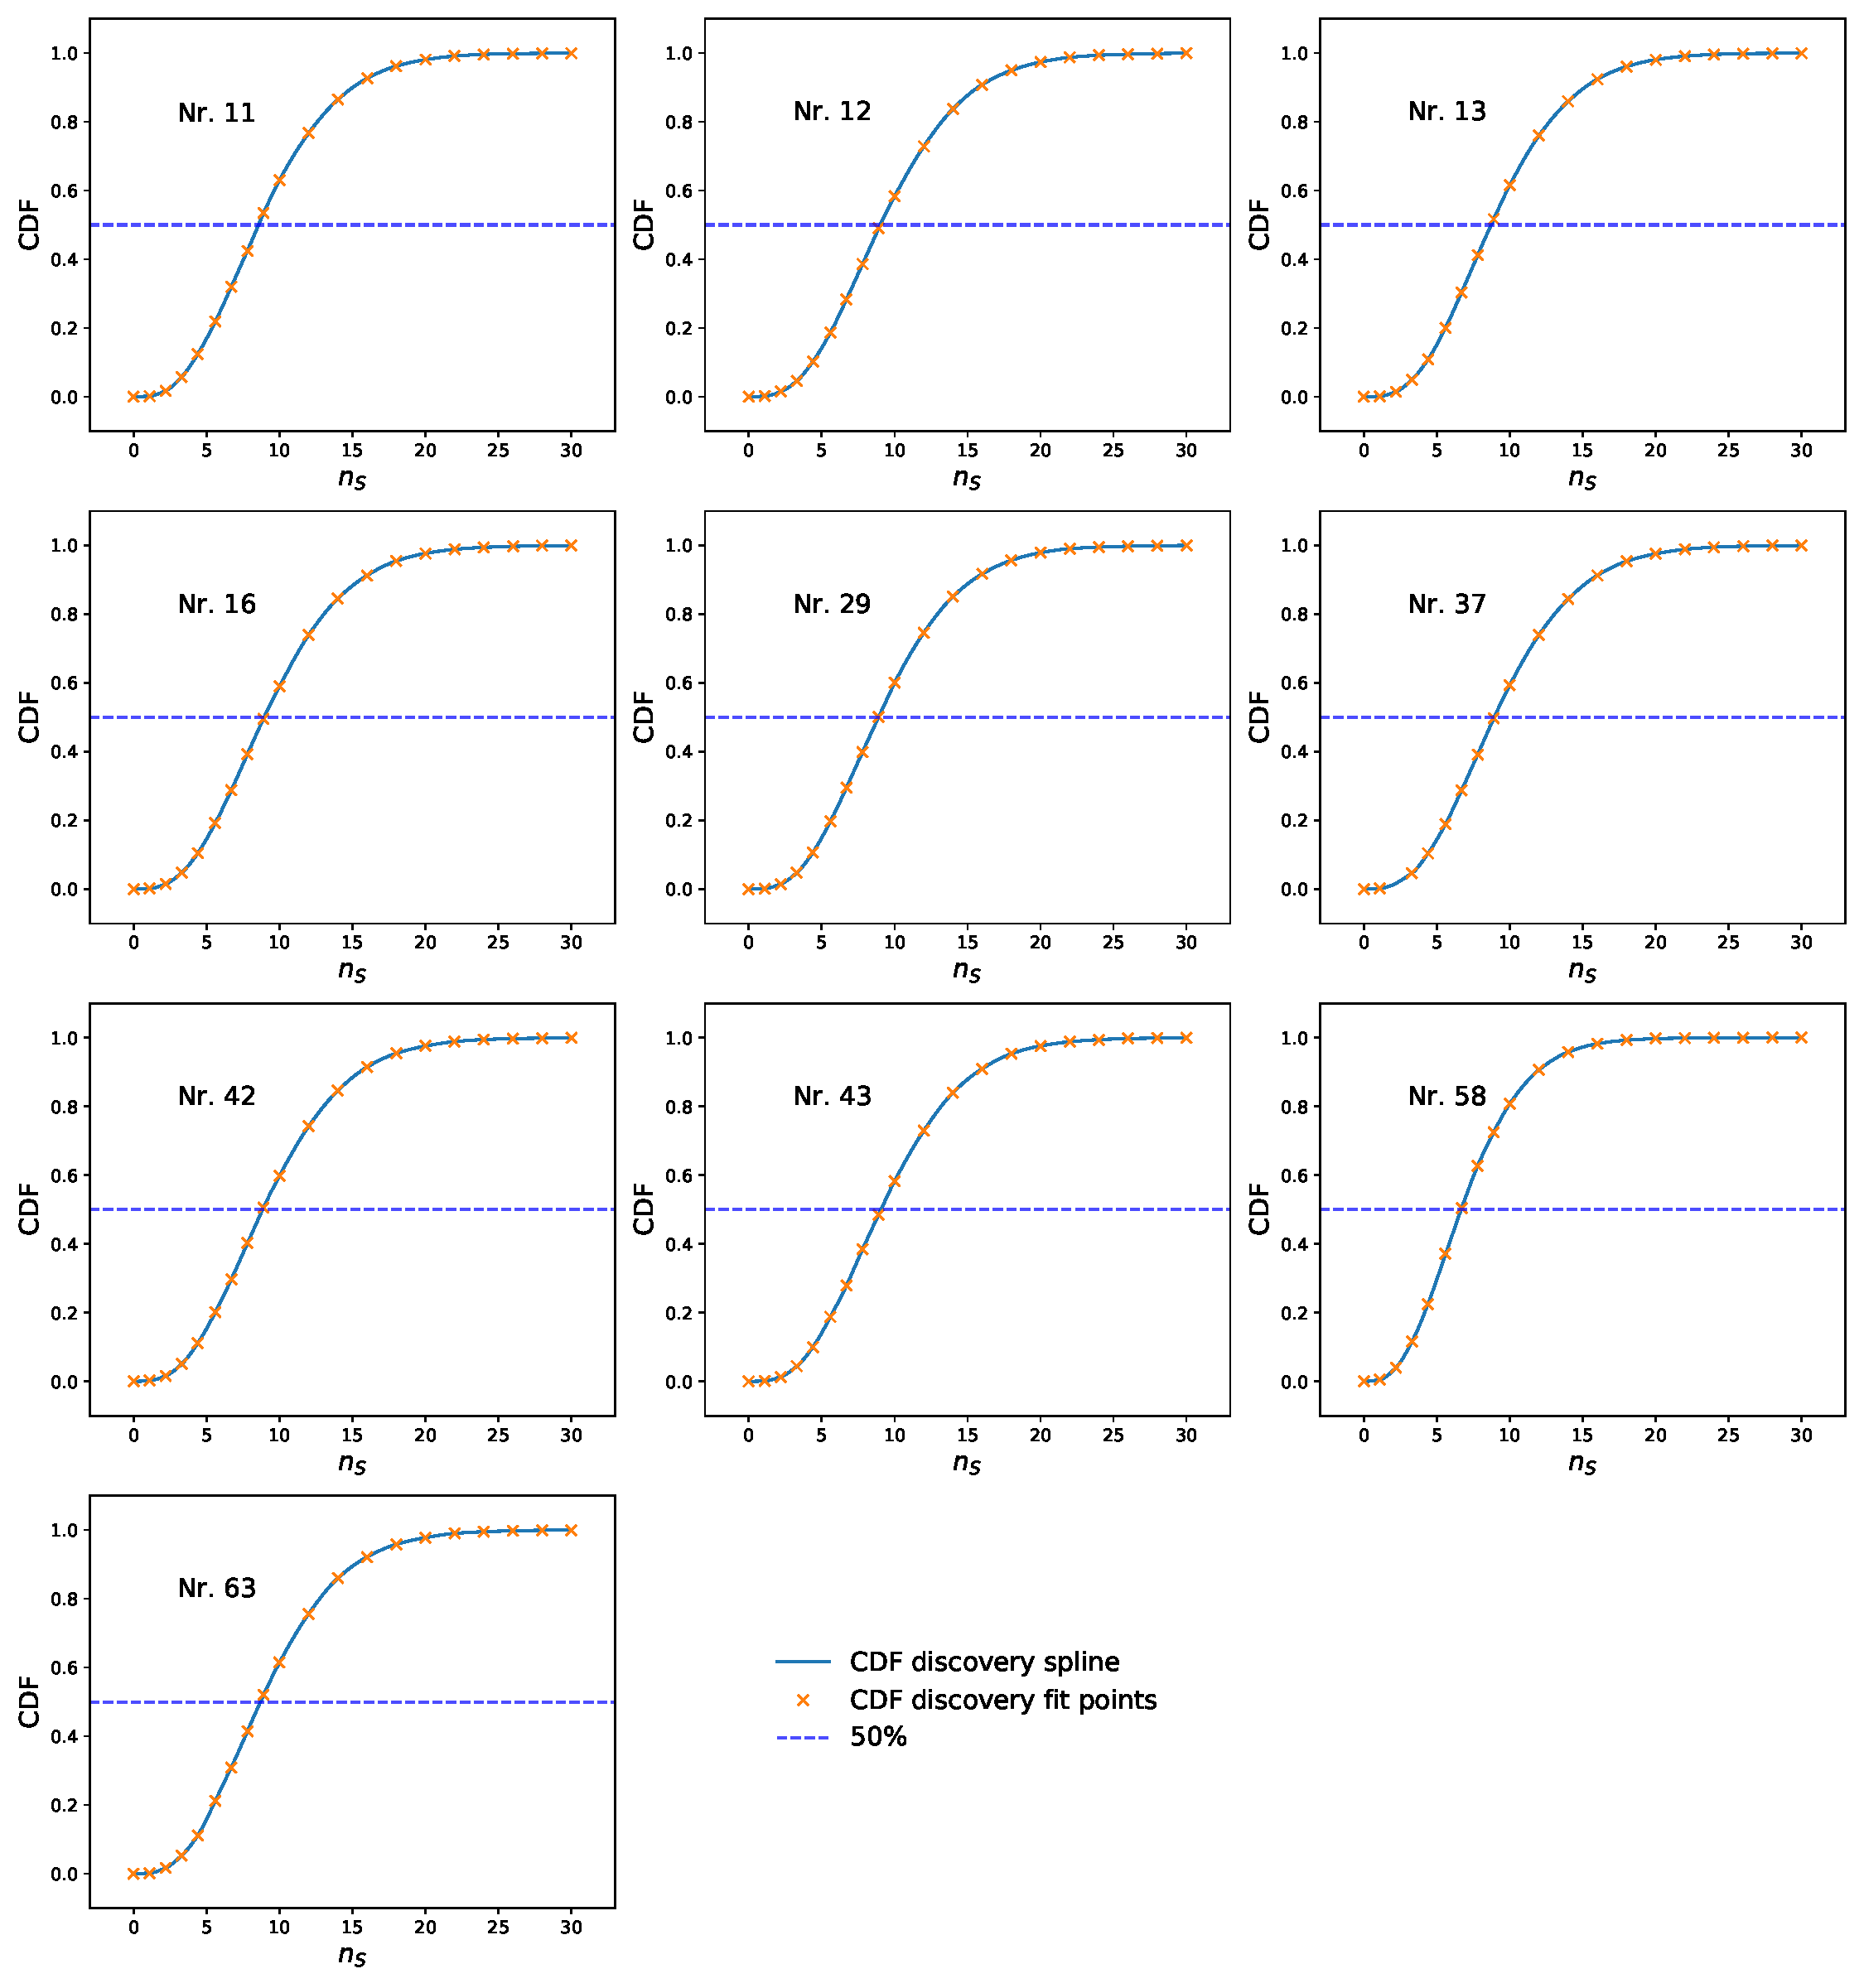
\includegraphics[width=\linewidth]{Plots/appendix/9_years_gfu_gold_time_dep_cdf_disc.pdf}
    \caption{Quantiles of the signal trials for the calculation of the discovery potential for the time-dependent analysis of all $\num{10}$ sources at a spectral index of $\gamma=\num{2}$. A $\chi^2$ CDF fit provides a more accurate estimate of the sought signal parameter $n_\text{S}$ which satisfies the condition of the discovery potential at $\SI{50}{\percent}$ represented via a dashed line.}
    \label{fig:time_dep_cdf_disc}
\end{figure}

\begin{figure}
    \centering
    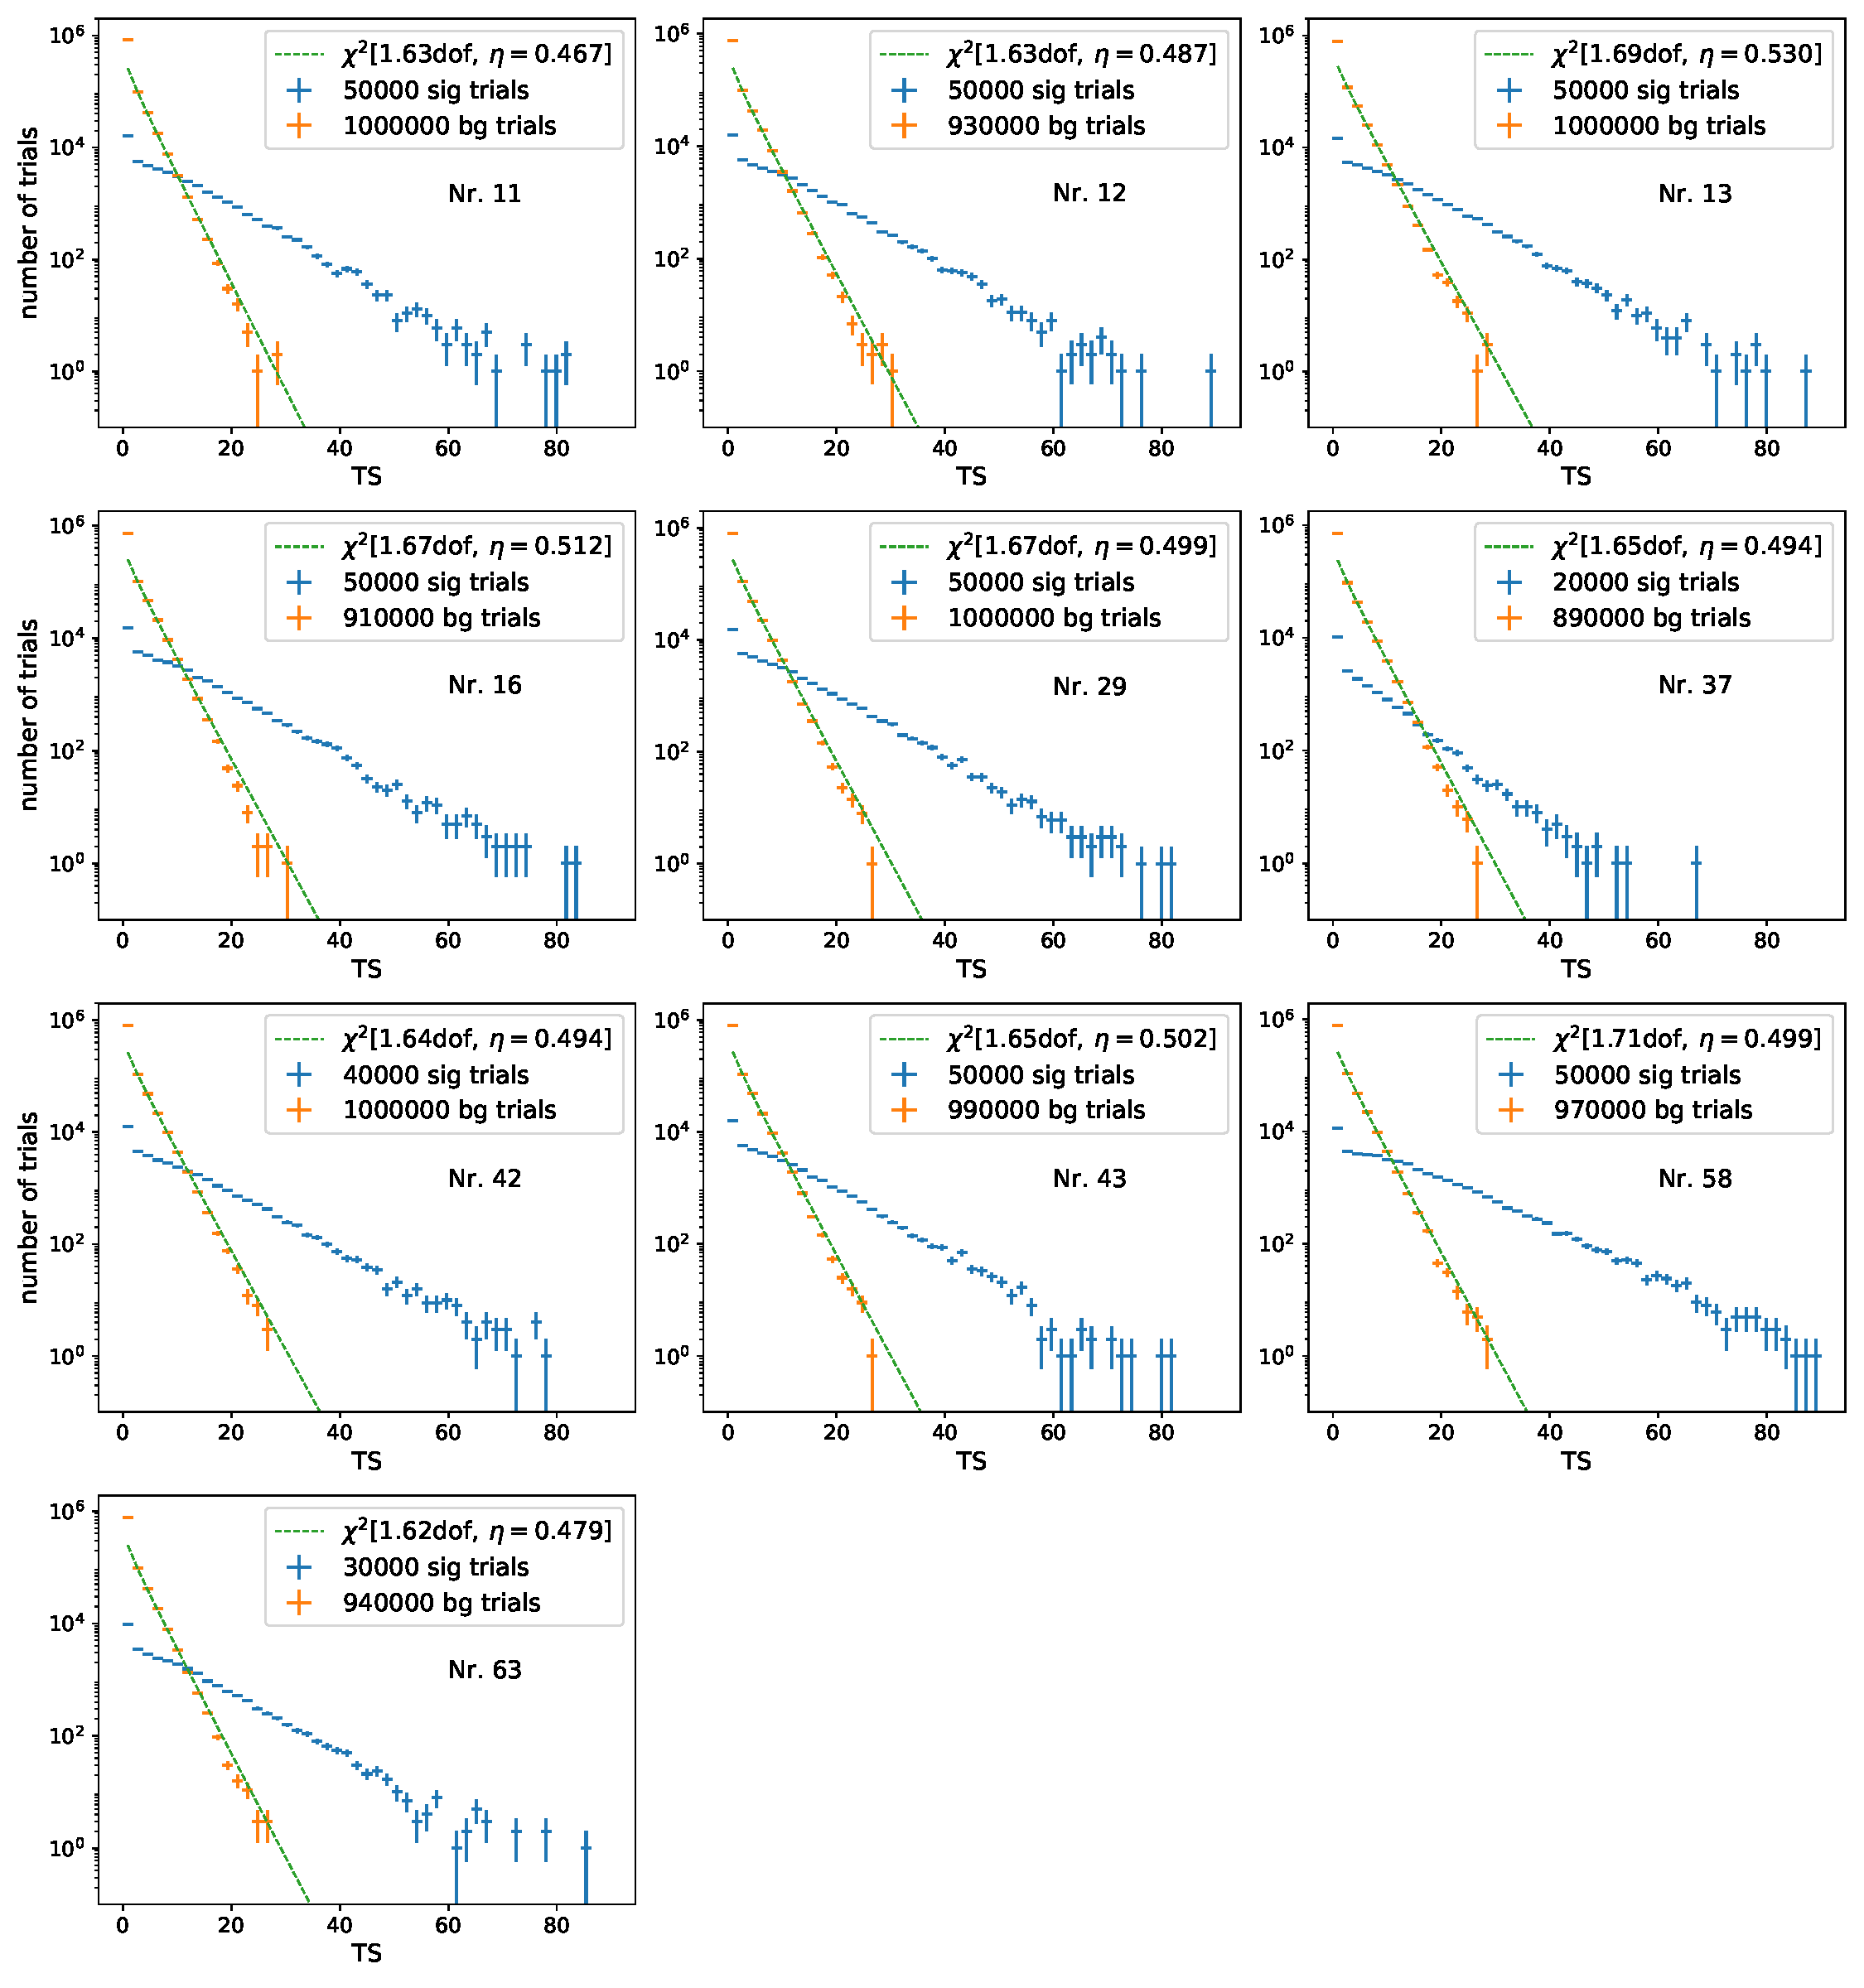
\includegraphics[width=\linewidth]{Plots/appendix/9_years_gfu_gold_time_dep_sig_sens_ts.pdf}
    \caption{Histogram of the background trials for the time-dependent analysis for all $\num{10}$ sources. Shown is also the set of signal trials with the number of injected signal events closest to satisfying the condition to calculate the sensitivity. The median of the background test statistics is not plotted as it is very close to the origin for all sources.}
    \label{fig:time_dep_sig_sens_ts}
\end{figure}

\begin{figure}
    \centering
    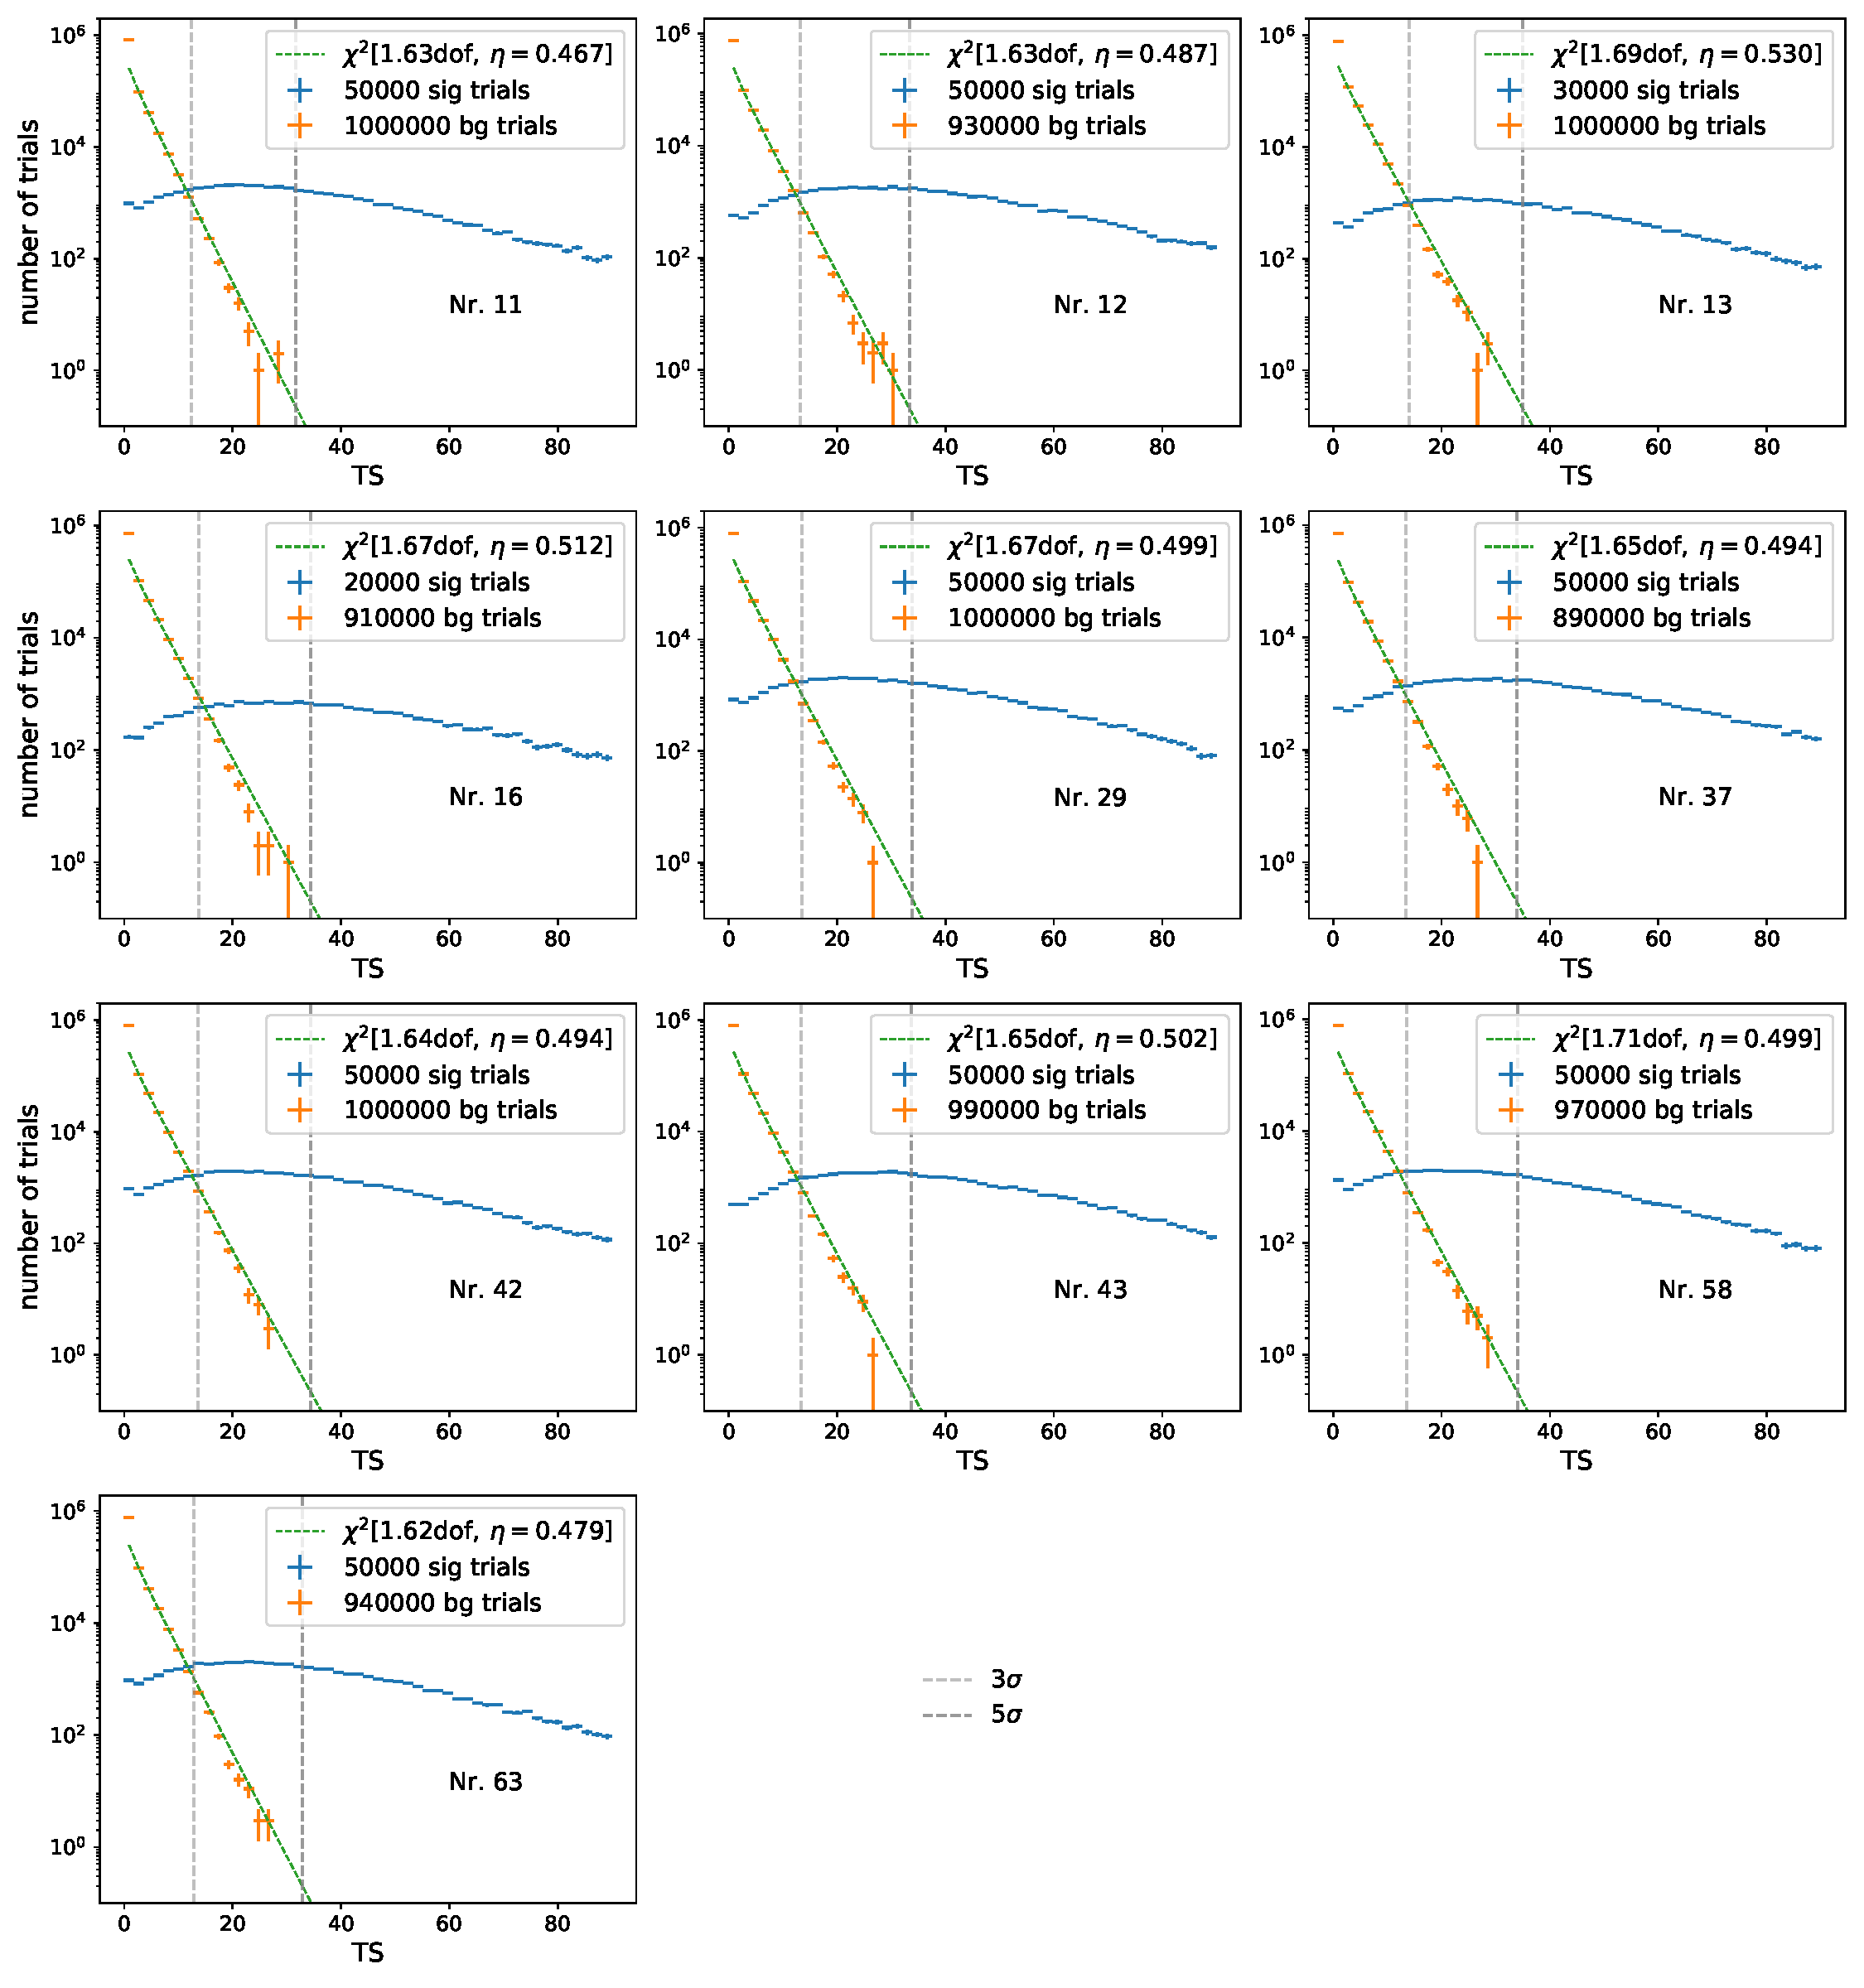
\includegraphics[width=\linewidth]{Plots/appendix/9_years_gfu_gold_time_dep_sig_disc_ts.pdf}
    \caption{Histogram of the background trials for the time-dependent analysis for all $\num{10}$ sources. Shown is also the set of signal trials with the number of injected signal events closest to satisfying the condition to calculate the discovery potential. The grey dashed lines represent $\num{3}\sigma$ and $\num{5}\sigma$ of the background teststatistic.}
    \label{fig:time_dep_sig_disc_ts}
\end{figure}

\begin{figure}
    \centering
    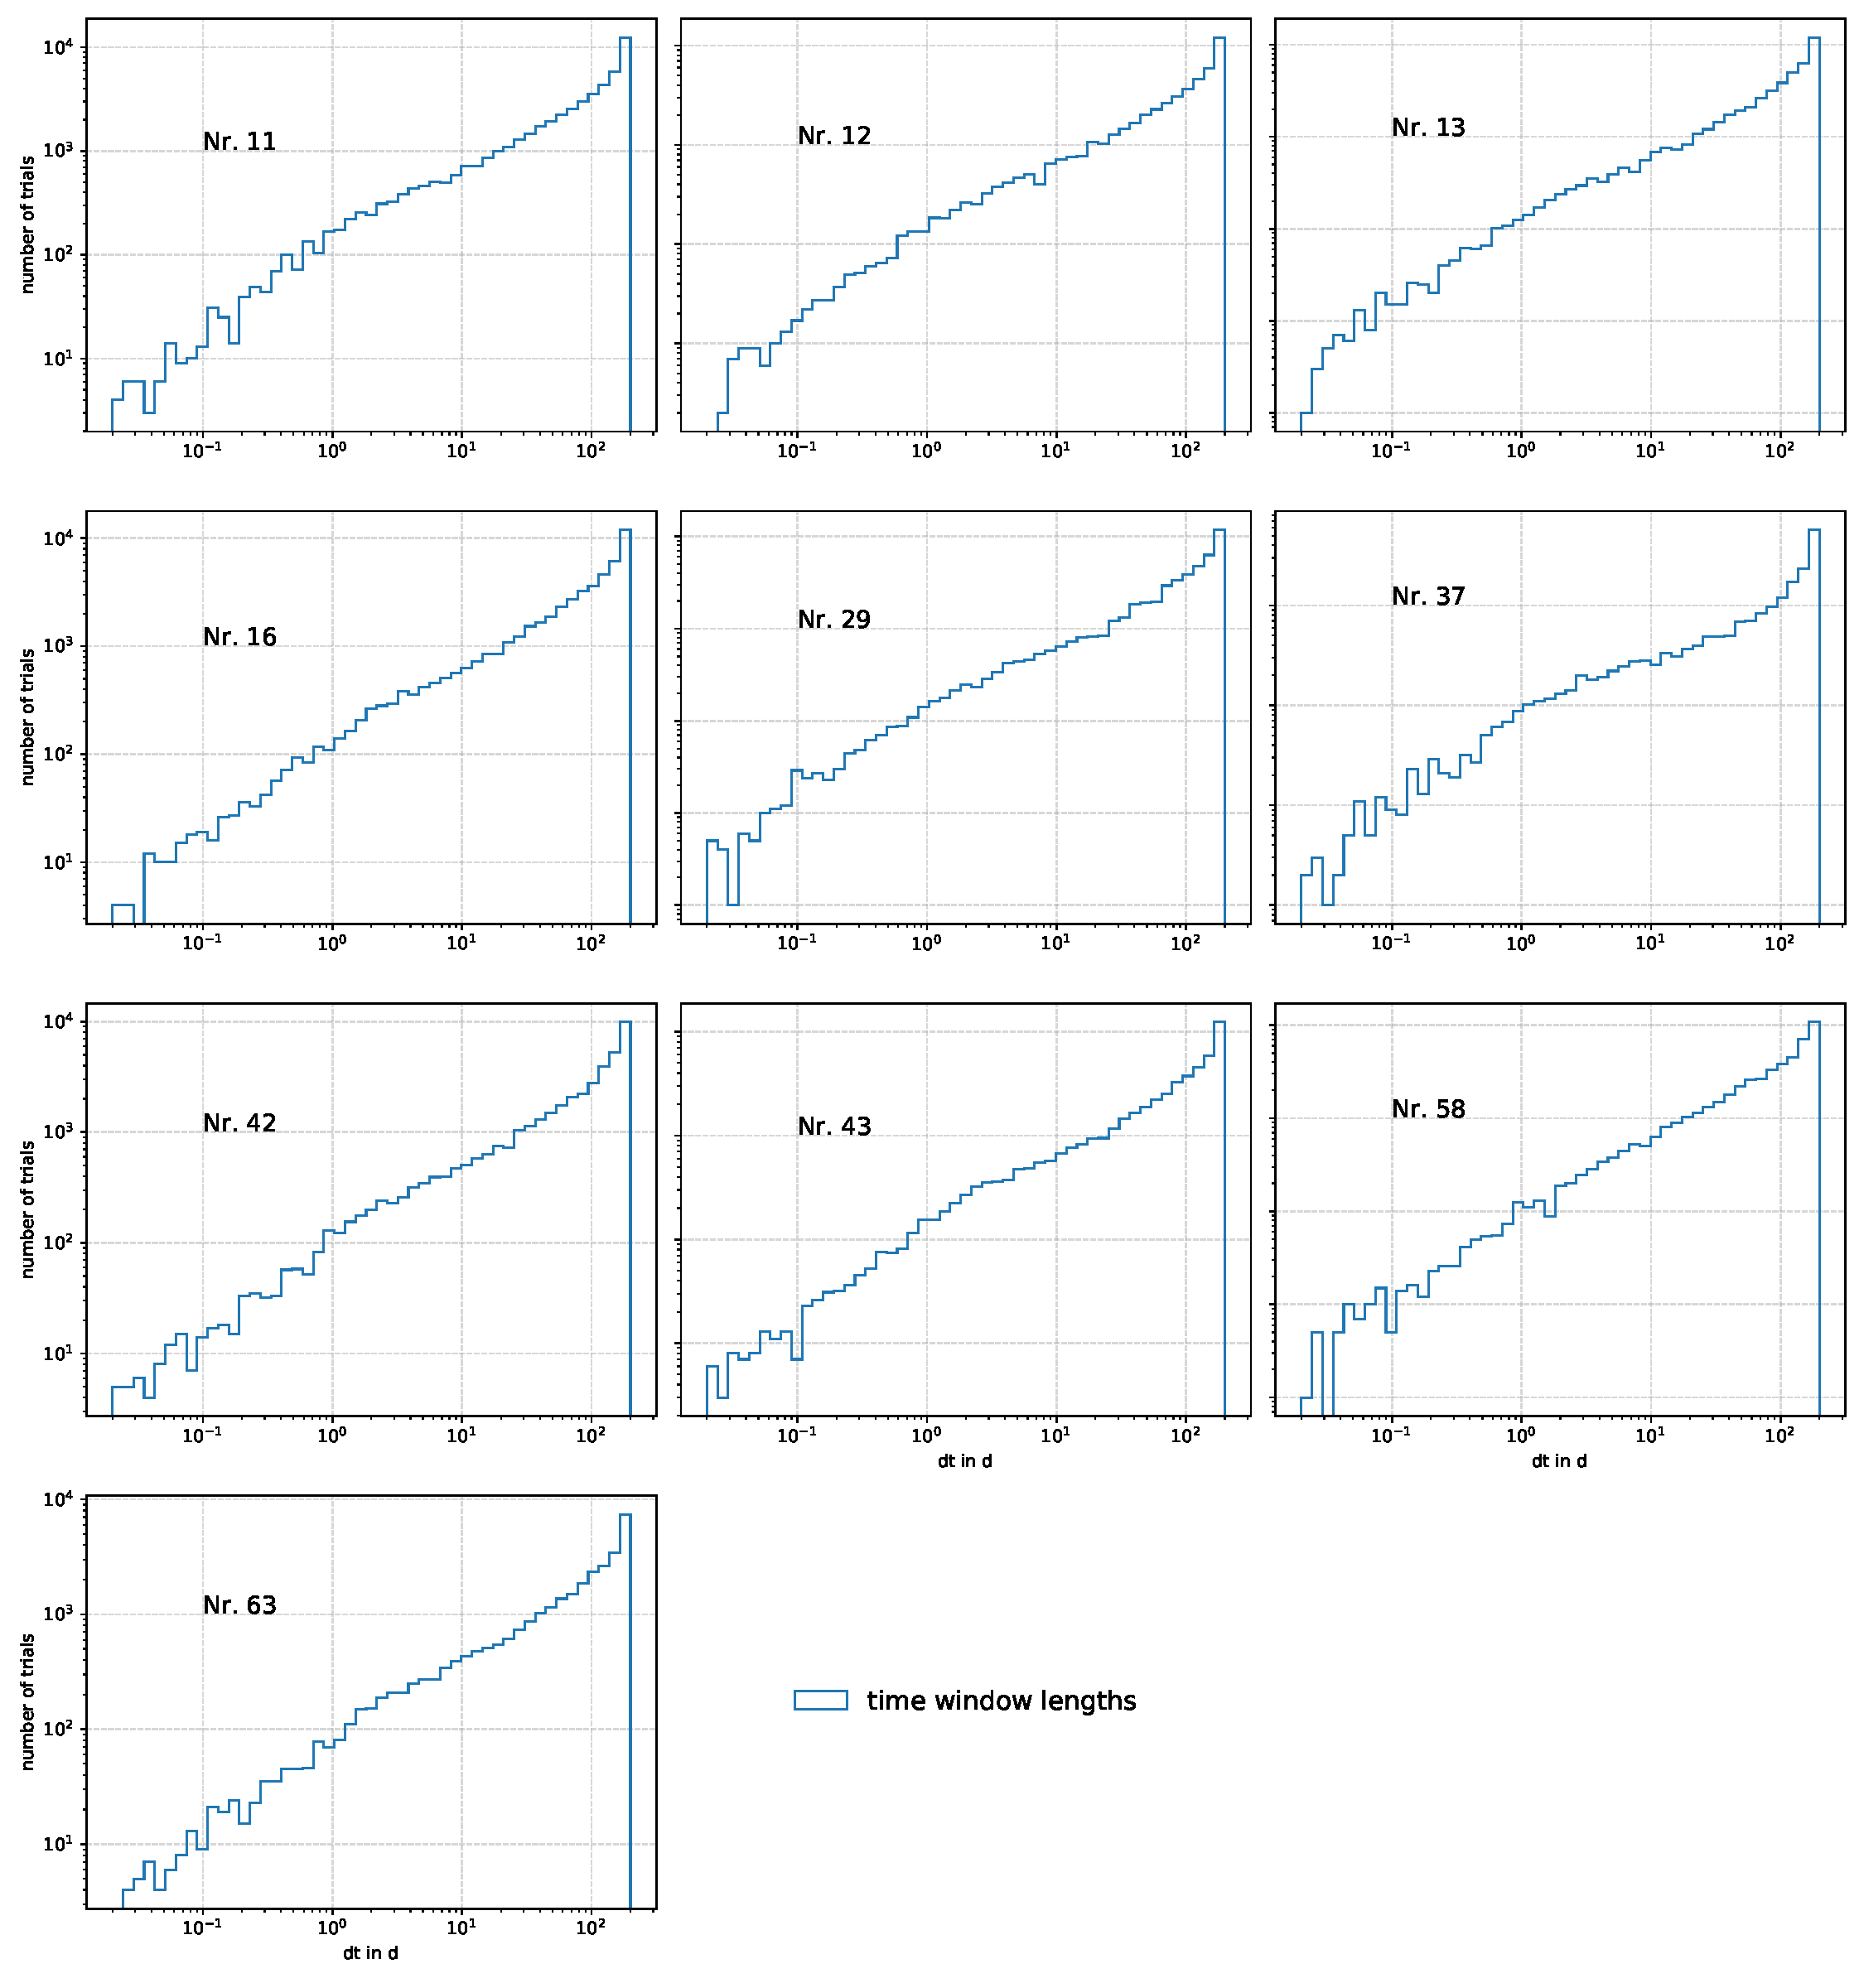
\includegraphics[width=\linewidth]{Plots/appendix/9_years_gfu_gold_time_dep_sens_dt.pdf}
    \caption{Histograms of the time window lengths $dt$ in days of all $\num{10}$ sources for the time-dependent analysis for the set of signal trials with the number of injected signal events closest to satisfying the condition to calculate the sensitivity.}
    \label{fig:sens_dt_all}
\end{figure}

\begin{figure}
    \centering
    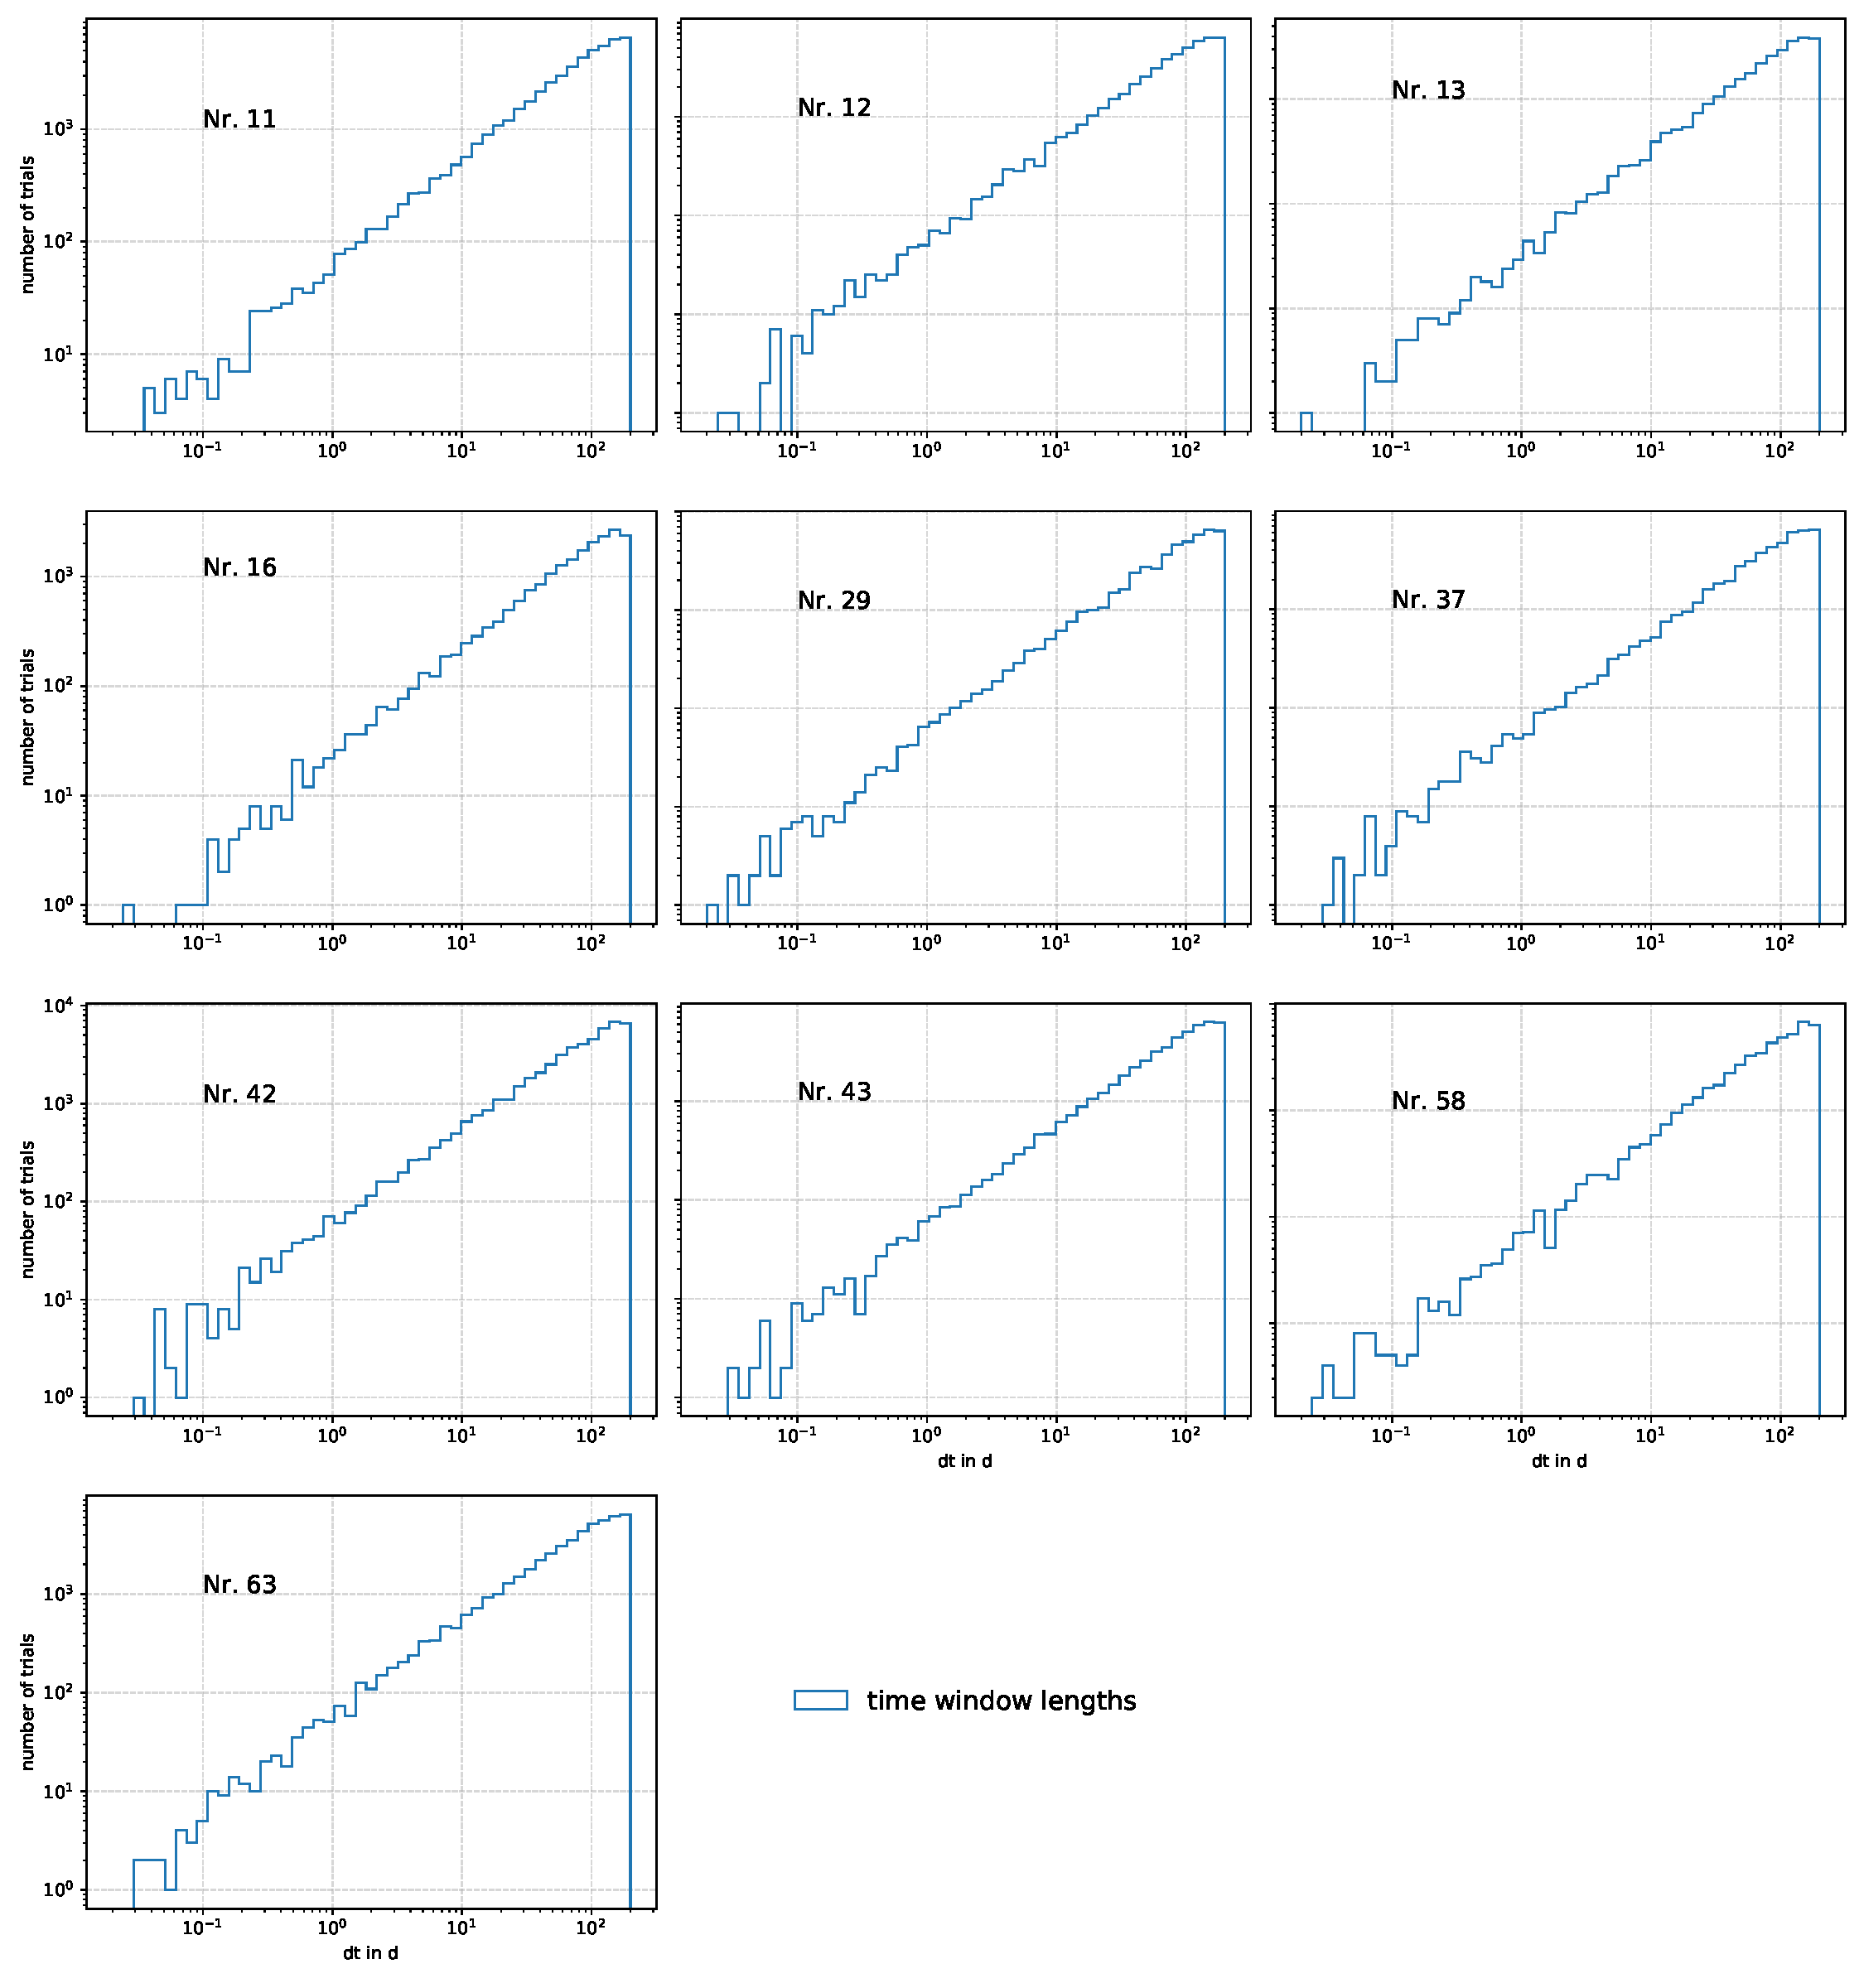
\includegraphics[width=\linewidth]{Plots/appendix/9_years_gfu_gold_time_dep_disc_dt.pdf}
    \caption{Histograms of the time window lengths $dt$ in days of all $\num{10}$ sources for the time-dependent analysis for the set of signal trials with the number of injected signal events closest to satisfying the condition to calculate the discovery potential.}
    \label{fig:disc_dt_all}
\end{figure}

\begin{figure}
    \centering
    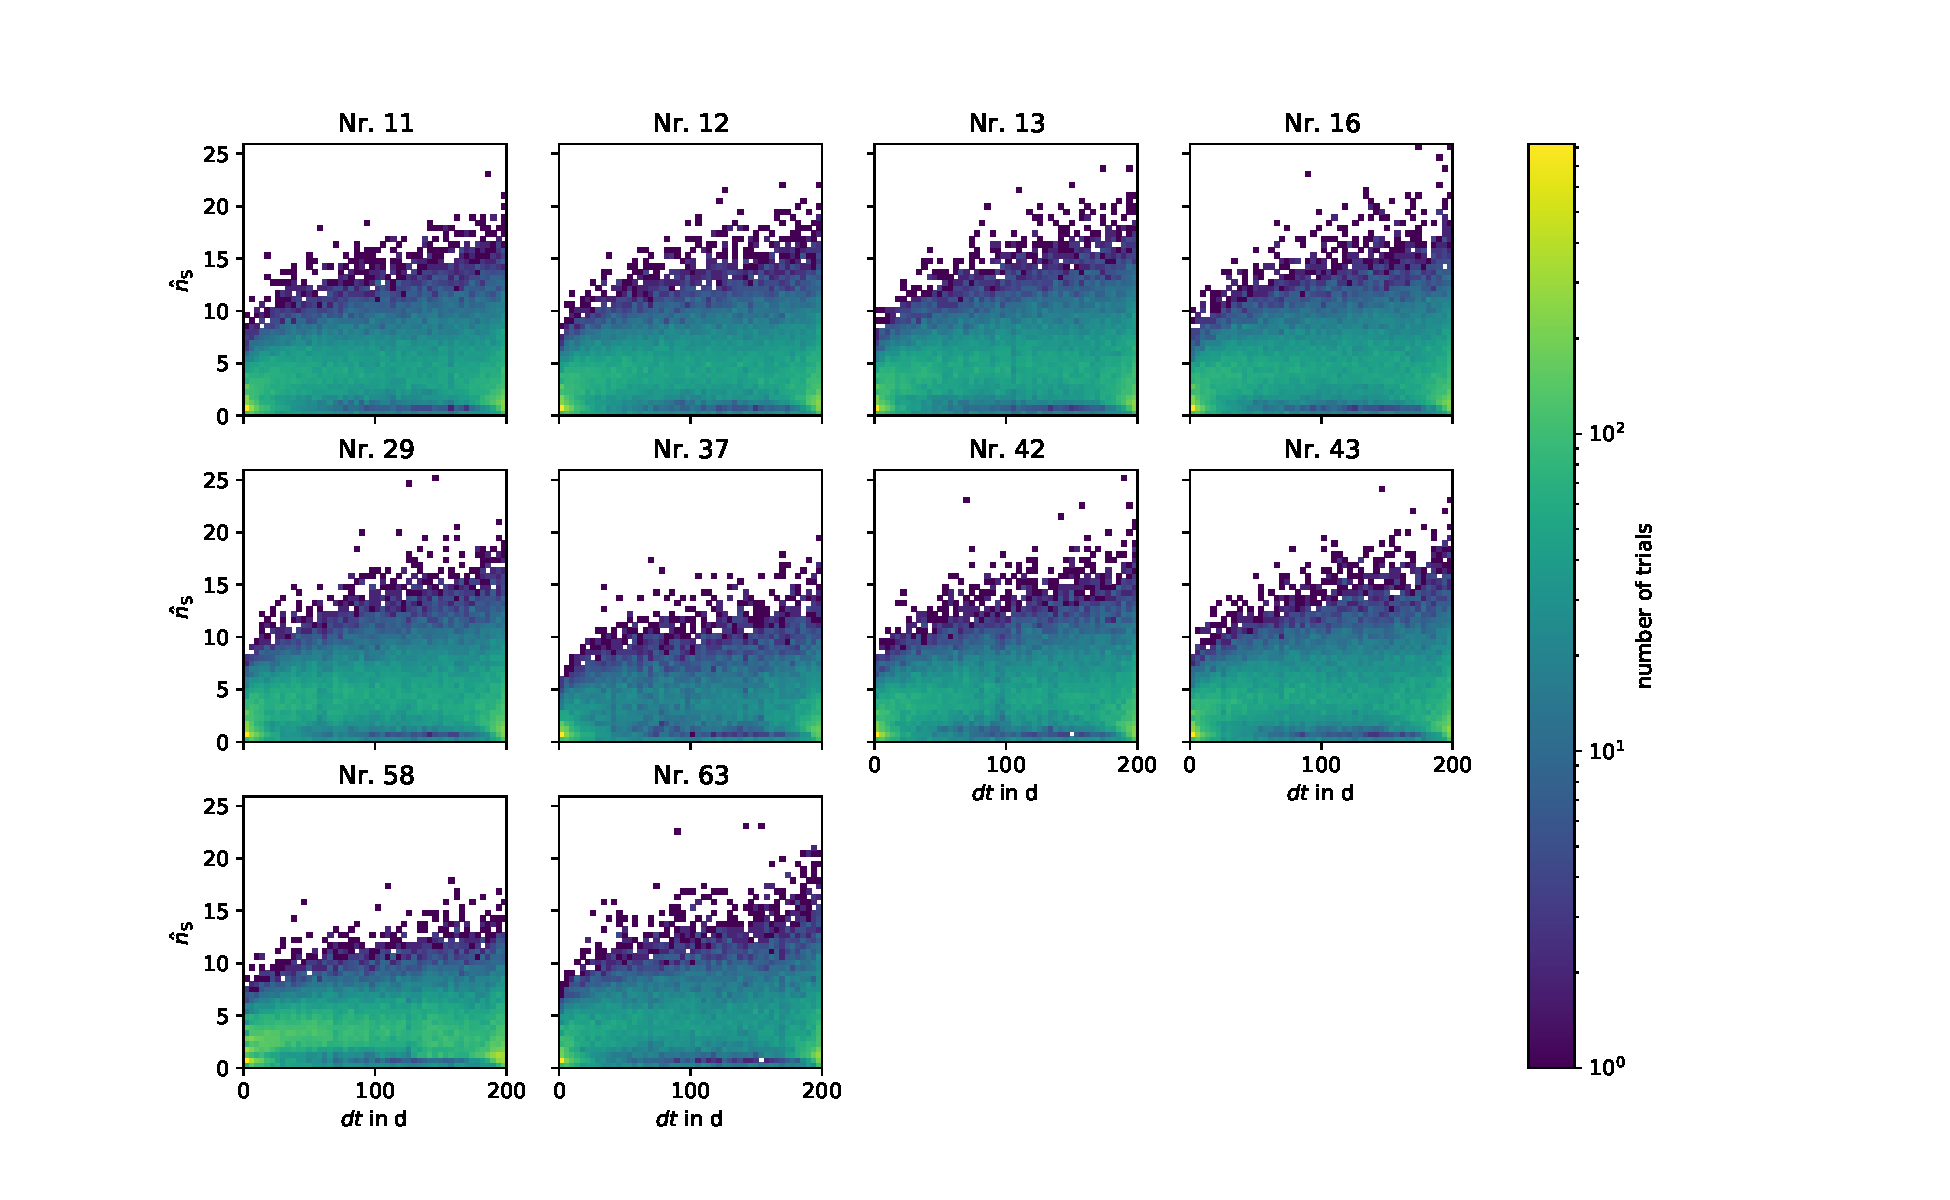
\includegraphics[width=\linewidth]{Plots/appendix/time_window_ns_sens_time_dep.pdf}
    \caption{Histograms of the time window lengths $dt$ in days in dependence of the fitted signal parameter $\hat{n}_\text{S}$ of all $\num{10}$ sources for the time-dependent analysis for the set of signal trials with the number of injected signal events closest to satisfying the condition to calculate the sensitivity.}
    \label{fig:sens_ns_dt_all}
\end{figure}

\begin{figure}
    \centering
    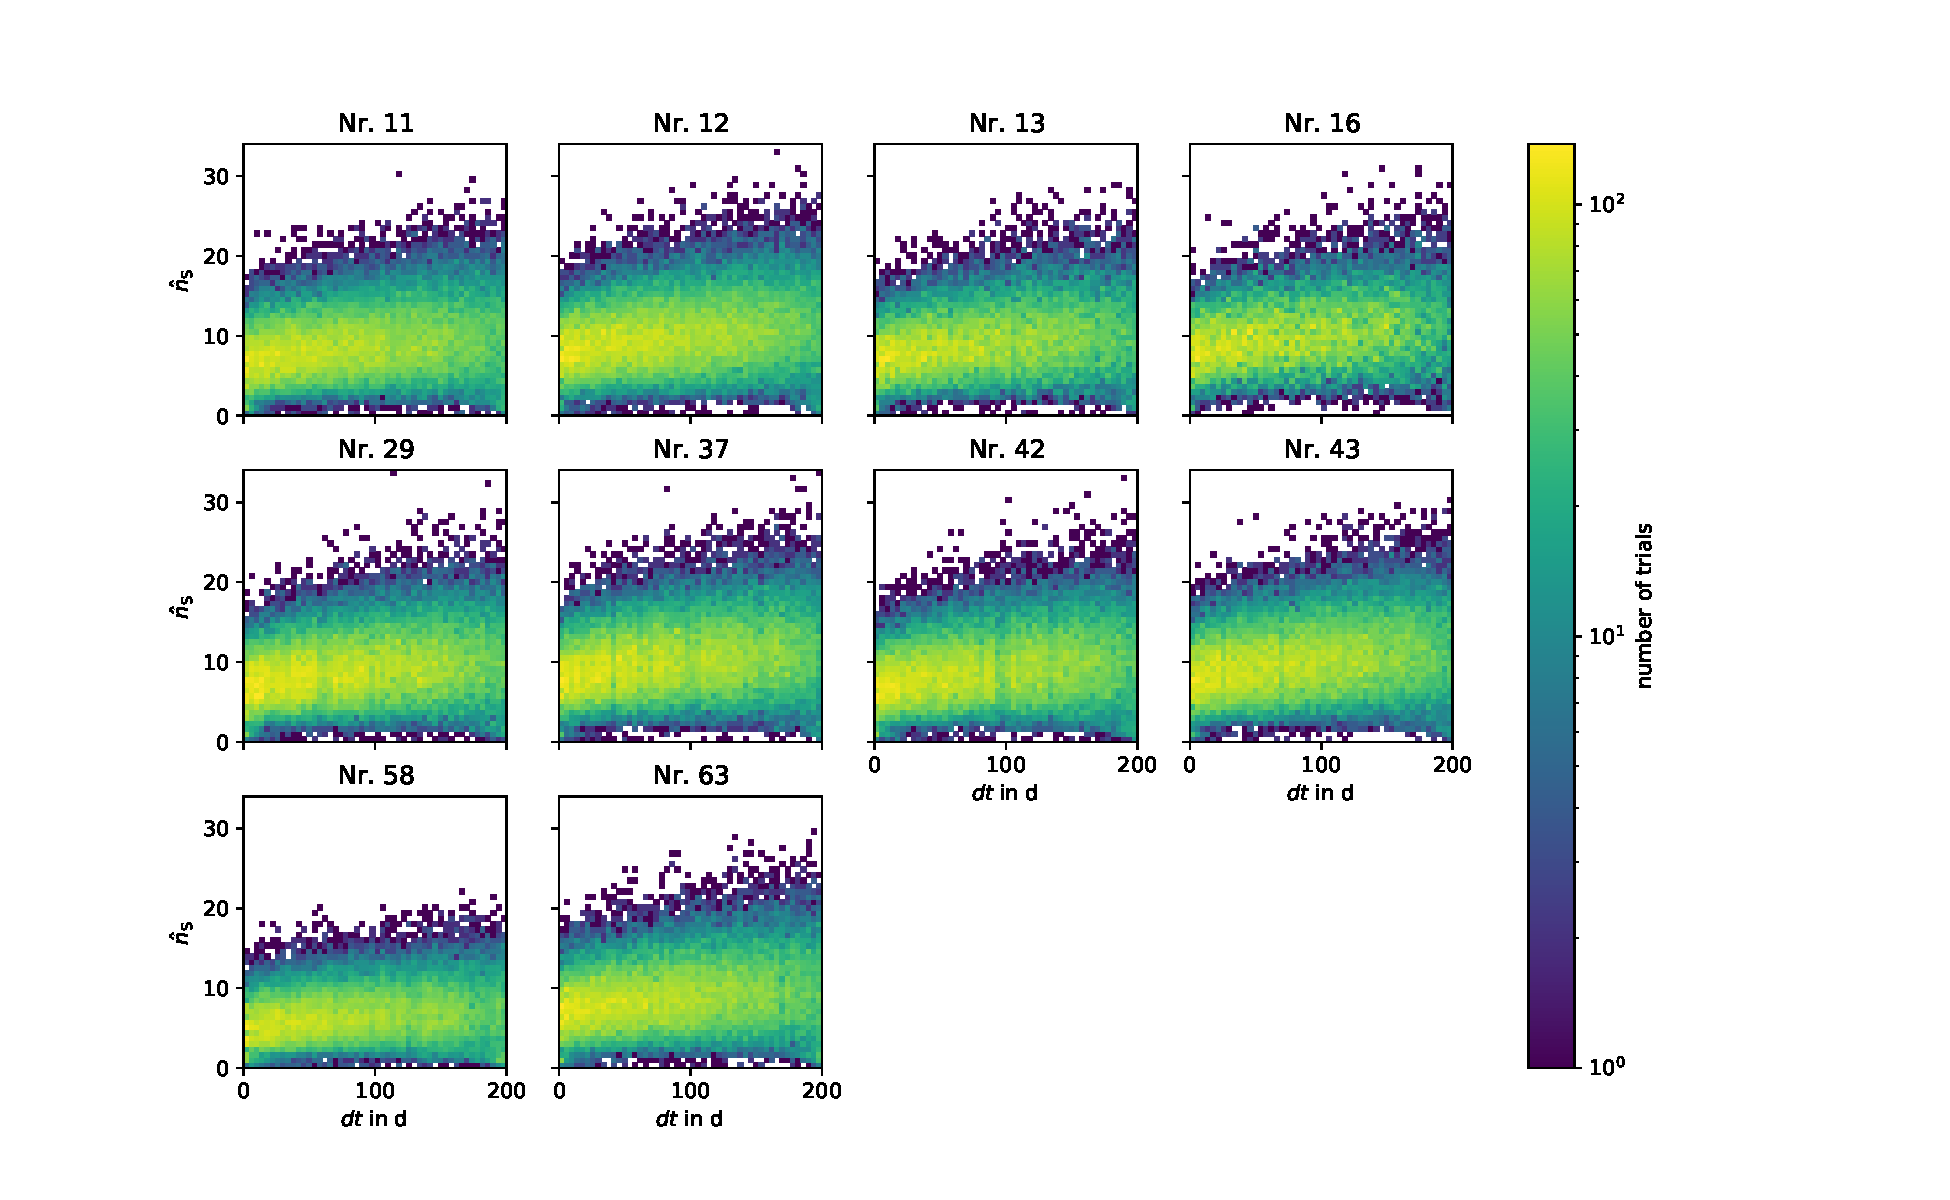
\includegraphics[width=\linewidth]{Plots/appendix/time_window_ns_disc_time_dep.pdf}
    \caption{Histograms of the time window lengths $dt$ in days in dependence of the fitted signal parameter $\hat{n}_\text{S}$ of all $\num{10}$ sources for the time-dependent analysis for the set of signal trials with the number of injected signal events closest to satisfying the condition to calculate the discovery potential.}
    \label{fig:disc_ns_dt_all}
\end{figure}

\newpage
\subsection{Examination of Fit Bias} \label{sec:fit_bias_time_dep}

\begin{figure}
    \centering
    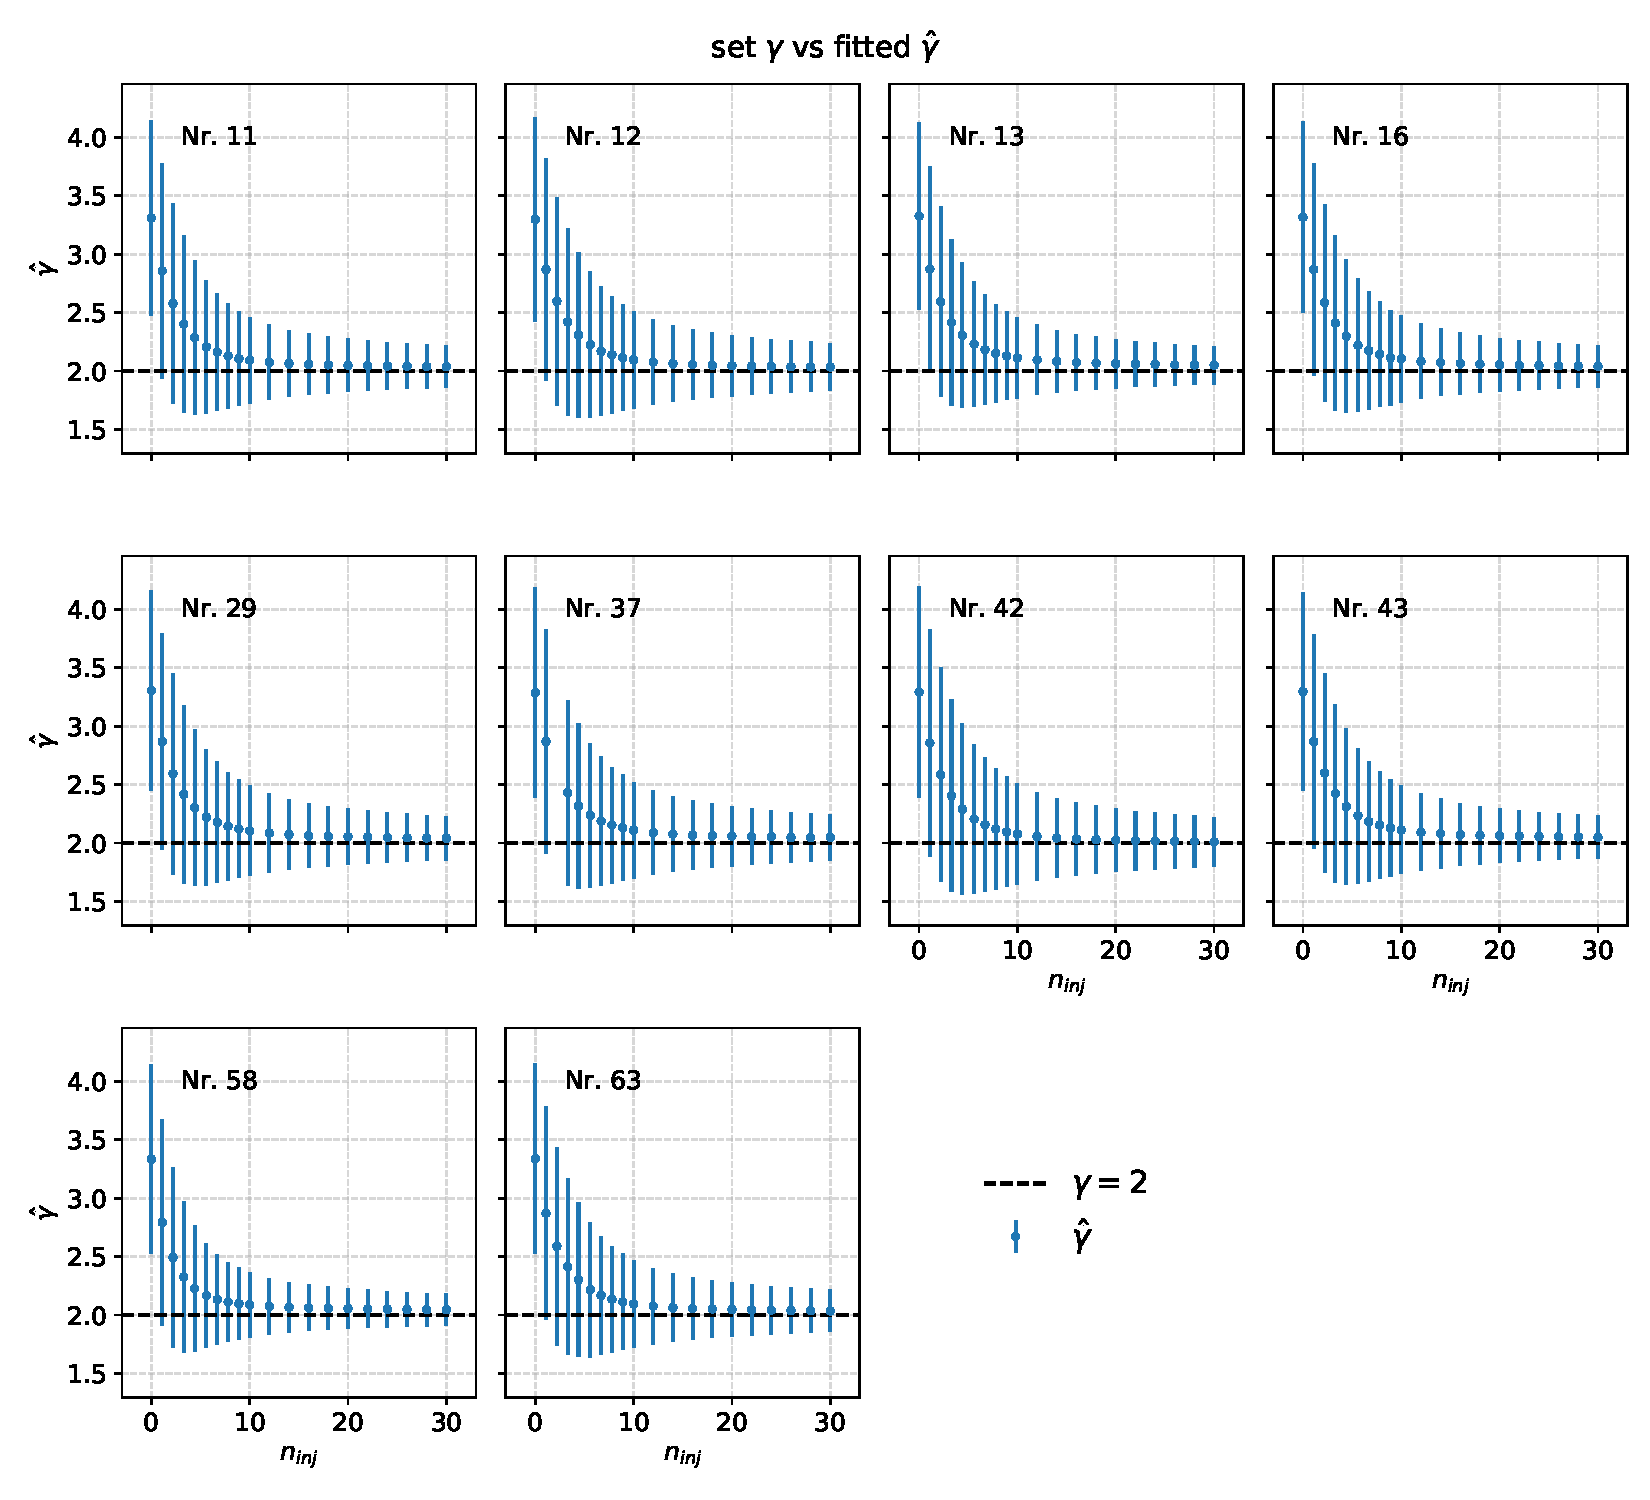
\includegraphics[width=\linewidth]{Plots/appendix/gamma_fit_time_dep.pdf}
    \caption{Fitted spectral index $\hat\gamma$ in dependence of the injected number of signal events $n_\text{inj}$ with spectral index $\gamma$, shown with a horizontal black dashed line, for the trials used in the time-dependent analysis.}
    \label{fig:gamma_fit_time_dep}
\end{figure}

\begin{figure}
    \centering
    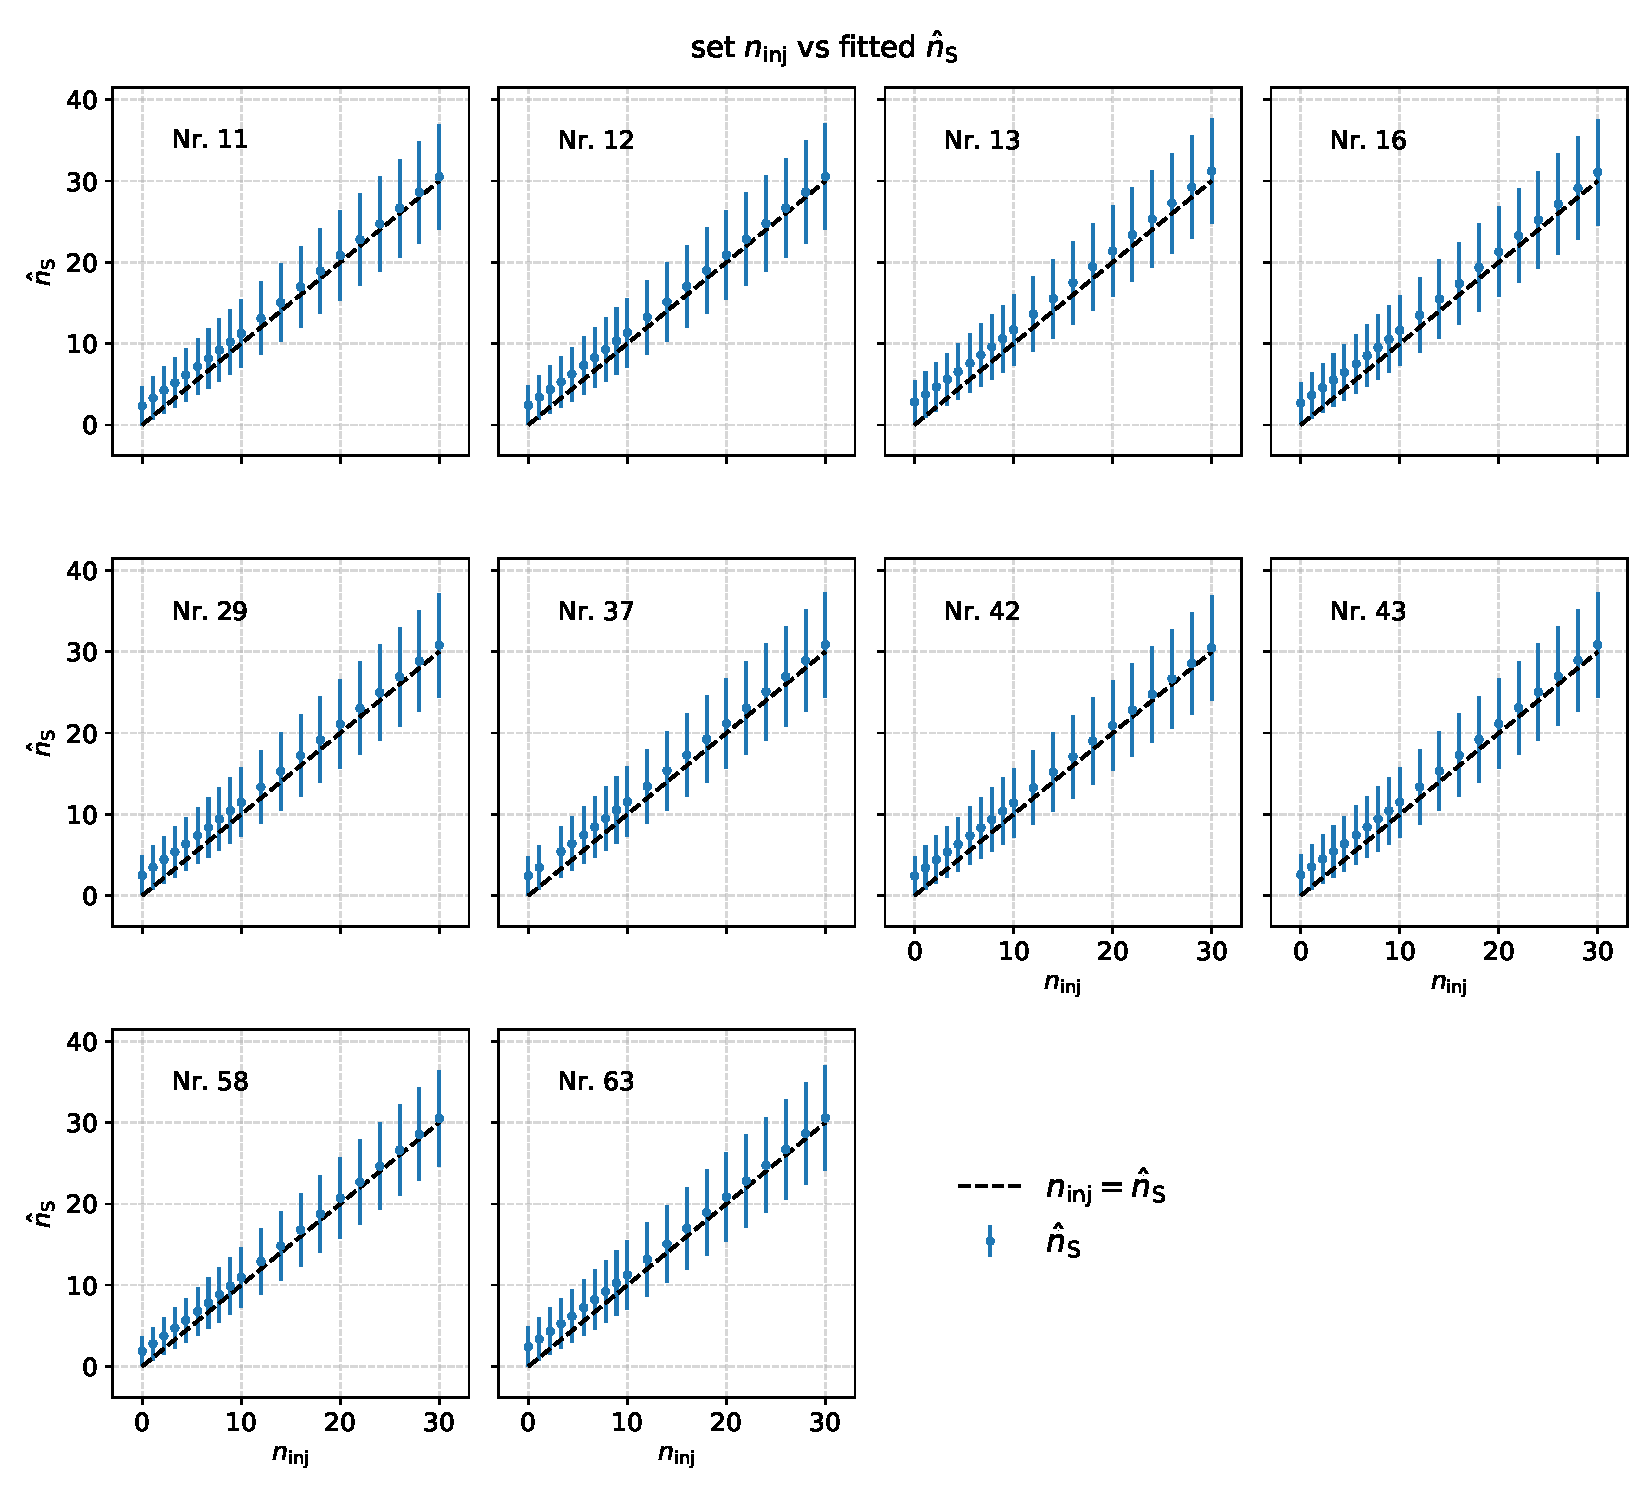
\includegraphics[width=\linewidth]{Plots/appendix/ns_fit_time_dep.pdf}
    \caption{Fitted number of signal events $\hat{n}_{\text{S}}$ in dependence of the injected number of signal events $n_\text{inj}$ with spectral index $\gamma$ for the time-dependent analysis. The black dashed line shows the equality of fitted and injected number of signal events.}
    \label{fig:ns_fit_time_dep}
\end{figure}

\section{Time-Dependent Stacking Software Approach}

This chapter contains additional understanding aids for the attempt to write software for point source searches.

\begin{figure}
  \scalebox{0.5}{
  \begin{tikzpicture}[scale=1]
    \node[draw] at (-10,2.5) {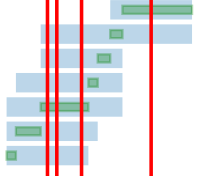
\includegraphics[width=4cm]{Plots/appendix/example.png}};
    % Koordinatensystem
    \draw[line width=0.25mm, ->] (-5,0) -- (-5,5);
    \draw[line width=0.25mm, ->] (-5,0) -- (10,0);
    \node at (10,-0.5) {time};
    \node at (-5.5,3) {rate};
    % Quellen
    \draw[line width=0.5mm, green] (-1,-1) -- (-1,4);
    \fill[pattern = north east lines, pattern color = green, opacity = 0.5,domain=-3:1,variable=\x]
    (-3,0)
    -- plot ({\x},{3.5})
    -- (1,0)
    -- cycle;
    \fill[pattern = north east lines, pattern color = green, opacity = 0.5,domain=-3:1,variable=\x]
    (-3,0)
    -- plot ({\x},{-0.5})
    -- (1,0)
    -- cycle;
    \draw[green] (-3,-0.5) -- (1,-0.5);
    \draw[green] (-3,3.5) -- (1,3.5);
    \draw[green] (-3,-0.5) -- (-3,3.5);
    \draw[green] (1,-0.5) -- (1,3.5);
    \node[green] at (-1,4.5) {$k=1$};

    \draw[line width=0.5mm, orange] (-0.8,-1) -- (-0.8,4);
    \fill[pattern = north east lines, pattern color = orange, opacity = 0.5,domain=-2.8:1.2,variable=\x]
    (-2.8,0)
    -- plot ({\x},{3.5})
    -- (1.2,0)
    -- cycle;
    \fill[pattern = north east lines, pattern color = orange, opacity = 0.5,domain=-2.8:1.2,variable=\x]
    (-2.8,0)
    -- plot ({\x},{-0.5})
    -- (1.2,0)
    -- cycle;
    \draw[orange] (-2.8,-0.5) -- (1.2,-0.5);
    \draw[orange] (-2.8,3.5) -- (1.2,3.5);
    \draw[orange] (-2.8,-0.5) -- (-2.8,3.5);
    \draw[orange] (1.2,-0.5) -- (1.2,3.5);
    \node[orange] at (-0.8,-1.5) {$k=2$};

    \draw[line width=0.5mm, red] (2.5,-1) -- (2.5,4);
    \fill[pattern = north west lines, pattern color = red, opacity = 0.5,domain=0.5:4.5,variable=\x]
    (0.5,0)
    -- plot ({\x},{3.5})
    -- (4.5,0)
    -- cycle;
    \fill[pattern = north west lines, pattern color = red, opacity = 0.5,domain=0.5:4.5,variable=\x]
    (0.5,0)
    -- plot ({\x},{-0.5})
    -- (4.5,0)
    -- cycle;
    \draw[red] (0.5,-0.5) -- (4.5,-0.5);
    \draw[red] (0.5,3.5) -- (4.5,3.5);
    \draw[red] (0.5,-0.5) -- (0.5,3.5);
    \draw[red] (4.5,-0.5) -- (4.5,3.5);
    \node[red] at (2.5,4.5) {$k=3$};

    \draw[line width=0.5mm, blue] (6,-1) -- (6,4);
    \fill[pattern = north east lines, pattern color = blue, opacity = 0.5, domain=4:8,variable=\x]
    (4,0)
    -- plot ({\x},{3.5})
    -- (8,0)
    -- cycle;
    \fill[pattern = north east lines, pattern color = blue, opacity = 0.5,domain=4:8,variable=\x]
    (4,0)
    -- plot ({\x},{-0.5})
    -- (8,0)
    -- cycle;
    \draw[blue] (4,-0.5) -- (8,-0.5);
    \draw[blue] (4,3.5) -- (8,3.5);
    \draw[blue] (4,-0.5) -- (4,3.5);
    \draw[blue] (8,-0.5) -- (8,3.5);
    \node[blue] at (6,4.5) {$k=4$};
    % Samples
    %\draw[line width=0.5mm] (6,-2) -- (6,5);
    %\draw[line width=0.5mm] (0,-2) -- (0,5);
    %\node at (-3,5) {j=1};
    %\node at (3,5) {j=2};
    %\node at (8,5) {j=3};
    % Events
    %\draw[line width=0.5mm,orange] (5,-2) -- (5,1);
    %\draw[line width=0.5mm,orange] (8,-2) -- (8,1);
    %\draw[line width=0.5mm,orange] (3,-2) -- (3,1);
    %\draw[line width=0.5mm,orange] (0.75,-1) -- (0.75,1);
    %\node at (0.9,-1.5) {\quad$0.5$};
    %\node at (3.1,-1.5) {\quad$1$};
    %\node at (5.1,-1.5) {\quad$0$};
    %\node at (8.1,-1.5) {\quad$1$};
    %\node[orange] at (0.75,-1.5) {$i=1$};
    %\node[orange] at (3,-2.5) {i=2};
    %\node[orange] at (5,-2.5) {i=1};
    %\node[orange] at (8,-2.5) {i=4};
    % Nodes
    %\node at (-1,-1.5) {$T_k(t_i)=$};
    %\node[gray] at (-5.8,1.5) {bg-rate};
    % sinus rate
    %\fill [pattern=north east lines,pattern color = blue, domain=2:6, variable=\x]
    %(2, 0)
    %-- plot ({\x}, {sin{(100*\x)}+2})
    %-- (6, 0)
    %-- cycle;
    %\fill [pattern=north east lines,pattern color = red, domain=5:6, variable=\x]
    %(5, 0)
    %-- plot ({\x}, {sin{(100*\x)}+1.5})
    %-- (6, 0)
    %-- cycle;
    %\draw[gray, thick,smooth,domain=0:6 , variable=\x] plot({\x},{0.5*sin{(100*\x)}+2});
    \draw[gray, line width=0.5mm, smooth,domain=-5:0, variable=\x] plot({\x},{0.5*sin{(100*\x)}+1.5});
    \draw[gray, line width=0.5mm, smooth,domain=0:5, variable=\x] plot({\x},{0.5*sin{(100*\x)}+1.5});
    \draw[gray, line width=0.5mm, smooth,domain=5:10, variable=\x] plot({\x},{0.5*sin{(100*\x)}+1.5});
    %\draw[gray, thick,smooth,domain=6:10, variable=\x] plot({\x},{0.5*sin{(100*\x)}+1});
    % intervals
    %\node at (2.5,7.25) {Old method: $\langle\lambda_{B,i=1}\rangle = \langle\lambda_{B,unique}\rangle$};
    %\draw[thick] (-3,7) -- (8,7);
    %\draw[thick] (-3,6.75) -- (-3,7.25);
    %\draw[thick] (8,6.75) -- (8,7.25);
    %\node at (0.75,6.25) {New method: $\langle\lambda_{B,i=1}\rangle = \langle\lambda_{B,\{k=1\cup k=2\}}\rangle$};
    %\draw[thick] (-3,6) -- (4.5,6);
    %\draw[thick] (-3,5.75) -- (-3,6.25);
    %\draw[thick] (4.5,5.75) -- (4.5,6.25);
    %thingie
    %\draw[thick, ->] (-5) -- (10);
    % arrow to picture
    \draw[very thick, ->, color=black] (-5.5,2.5) -- (-7,2.5);
  \end{tikzpicture}}
  \caption{This figure shows a scenario of $\num{4}$ sources $k$ with their timewindows (dashed areas). Each unique temporal position translates into a green area on the left, so does a source with a red line. Each green interval is the activation region indicating that an event falling into that region gets compared to an estimated background created in the underlying light blue temporal interval. The scenario therefore generates $\num{7}$ different models. The grey line shows the background rate with its seasonal variations.}
  \label{fig:activation}
\end{figure}

\chapter{Reproduction}

This chapter contains all the necessary information to reproduce the analyses.

\section{Main Analyses}

The analyse repo can be found at (git link).
The analysis was written on the external server cobalt and is located at (analysis folder).
It was written in \textbf{Python3} version 3.7.5 and uses \textbf{csky} version 1.1.7.
To compile it, the shell under (shell directory) was used.
This shell contains all the necessary dependencies to run the analysis.
In order to be able to reproduce the analysis, the directories in the \textbf{\_paths.py} file must first be adapted to the user.
The analysis should be done in three main steps, the data preparation, the time-integrated analysis and the time-dependent analysis.

\subsection{Data Preparation}
The first step is to create the source files for the neutrino sources through the \textbf{make\_source\_files\_from\_fits.py} file.
The skymaps are created by the file \textbf{make\_skymap.py}.
This is followed by the creation of the preprocessed datasets.
The script \textbf{check\_gold\_filter\_jobs.py} creates job files which can be processed on the server condor, these use the script \textbf{check\_gold\_mc\_ids.py} and can be started in the job folder with the bash command on condor (here: \textbf{bash ehe\_transient\_stacking.dag.start.sh}).
Once the scripts have run, they can be collected via \textbf{check\_gold\_filter\_combine.py}.
These datasets can now be inserted into \textbf{csky} into the \textbf{selections.py} file via creating a new dataset class.

\begin{verbatim}
class my_cleaned_data(PSDataSpec):
    _user_path = os.path.join("/data","user","jkollek","csky_ehe_stacking",
                              "rawout_tests","cleaned_datasets_new")
    _path_sig = os.path.join(_user_path,'IC86_2016_MC.npy')
    _path_data = [os.path.join(_user_path,'IC86_2011_exp.npy'),
                  os.path.join(_user_path,'IC86_2012_exp.npy'),
                  os.path.join(_user_path,'IC86_2013_exp.npy'),
                  os.path.join(_user_path,'IC86_2014_exp.npy'),
                  os.path.join(_user_path,'IC86_2015_exp.npy'),
                  os.path.join(_user_path,'IC86_2016_exp.npy'),
                  os.path.join(_user_path,'IC86_2017_exp.npy'),
                  os.path.join(_user_path,'IC86_2018_exp.npy'),
                  os.path.join(_user_path,'IC86_2019_exp.npy')]
    _path_grls = [os.path.join(_user_path,'GRL','IC86_2011_exp.npy'),
                  os.path.join(_user_path,'GRL','IC86_2012_exp.npy'),
                  os.path.join(_user_path,'GRL','IC86_2013_exp.npy'),
                  os.path.join(_user_path,'GRL','IC86_2014_exp.npy'),
                  os.path.join(_user_path,'GRL','IC86_2015_exp.npy'),
                  os.path.join(_user_path,'GRL','IC86_2016_exp.npy'),
                  os.path.join(_user_path,'GRL','IC86_2017_exp.npy'),
                  os.path.join(_user_path,'GRL','IC86_2018_exp.npy'),
                  os.path.join(_user_path,'GRL','IC86_2019_exp.npy')]
    _bins_sindec = np.unique(np.concatenate([
                        np.linspace(-1, -0.93, 4 + 1),
                        np.linspace(-0.93, -0.3, 10 + 1),
                        np.linspace(-0.3, 0.05, 9 + 1),
                        np.linspace(0.05, 1, 18 + 1) ]) )
    _bins_logenergy = np.arange(1, 9.5 + 0.01, 0.125)
\end{verbatim}

\subsection{Time-integrated Analysis}

\subsection{Time-dependent Analysis}

\section{Time-Dependent Stacking Software Approach}
